\documentclass[9pt,twocolumn,twoside]{osajnl}


\usepackage{times}

\usepackage{amsmath}
\usepackage{amssymb}
\usepackage{multirow}
\usepackage{multirow}
\usepackage{mathtools}
\usepackage{units}
\usepackage{subfloat}
\usepackage{float}
\usepackage[]{units}
\usepackage{xcolor}
\usepackage{url}
\usepackage{bbm}
\usepackage{algorithm}
\usepackage{algpseudocode}
\usepackage{pbox}
\usepackage{placeins}

\journal{ol}

\setboolean{shortarticle}{false}

\title{在挑战性地形上学习四足运动（Learning Quadrupedal Locomotion over Challenging Terrain）}

\author[1,*]{Joonho Lee}
\author[1,2,$\dagger$]{Jemin Hwangbo}
\author[1]{Lorenz Wellhausen}
\author[3]{Vladlen Koltun}
\author[1]{Marco Hutter}

\affil[1]{Robotic Systems Lab, ETH Zurich, Zurich, Switzerland}
\affil[2]{Robotics and Artificial Intelligence Lab, KAIST, Daejeon, Korea}
\affil[3]{Intelligent Systems Lab, Intel, Santa Clara, CA, USA}
\affil[$\dagger$]{本工作的主要部分在其于单位1访问期间完成}
\affil[*]{通讯作者（Corresponding author）: jolee@ethz.ch}

\dates{本文为 Science Robotics Vol. 5, Issue 47, eabc5986 (2020) 的接收版本 \\ DOI: 10.1126/scirobotics.abc5986}
% \dates{This is the accepted version of Science Robotics Vol. 5, eabc5986 (2020)}

\begin{abstract}
地球上一些最具挑战性的环境对于四足动物而言是可以到达的，但自主机器却无法进入。腿足运动（Legged Locomotion）能够极大地扩展机器人学的操作领域。然而，传统的腿足运动控制器基于精心设计的状态机（State Machine），显式触发运动基元（Motion Primitive）和反射的执行。这些设计的复杂性不断增加，但在通用性和鲁棒性方面仍不及动物的运动能力。本文提出了一种在挑战性自然环境中进行腿足运动的极其鲁棒的控制器。本文提出了一种将本体感知（Proprioception）反馈整合到运动控制中的新颖解决方案，并展示了从仿真（Simulation）到自然环境的卓越零样本泛化（Zero-Shot Generalization）能力。该控制器通过在仿真中的强化学习（Reinforcement Learning, RL）进行训练，其核心是一个作用于本体感知信号流的神经网络。训练好的控制器已带领两代四足ANYmal机器人进入了各种自然环境，这些环境超越了先前发表的腿足运动研究成果所能达到的范围。在训练中从未遇到过的条件下，该控制器仍能保持鲁棒性：可变形地形（Deformable Terrain）（如泥地和雪地）、动态落足点（Dynamic Foothold）（如碎石堆）以及地面障碍物（如茂密植被和汹涌水流）。本文的工作为机器人学开辟了新前沿，并表明通过在更简单的领域中训练即可在自然环境中实现极致的鲁棒性。
\end{abstract}


% Chinese support (auto-injected)
\usepackage{xeCJK}
\setCJKmainfont{Noto Serif CJK SC}[ItalicFont=AR PL UKai TW MBE]
\setCJKsansfont{Noto Sans CJK SC}
\setCJKmonofont{Noto Sans CJK SC}
\raggedbottom
\renewcommand{\figurename}{图}
\renewcommand{\tablename}{表}
\renewcommand{\abstractname}{摘要}
\renewcommand{\refname}{参考文献}
\begin{document}

\maketitle
\begin{figure*}
    \centering
    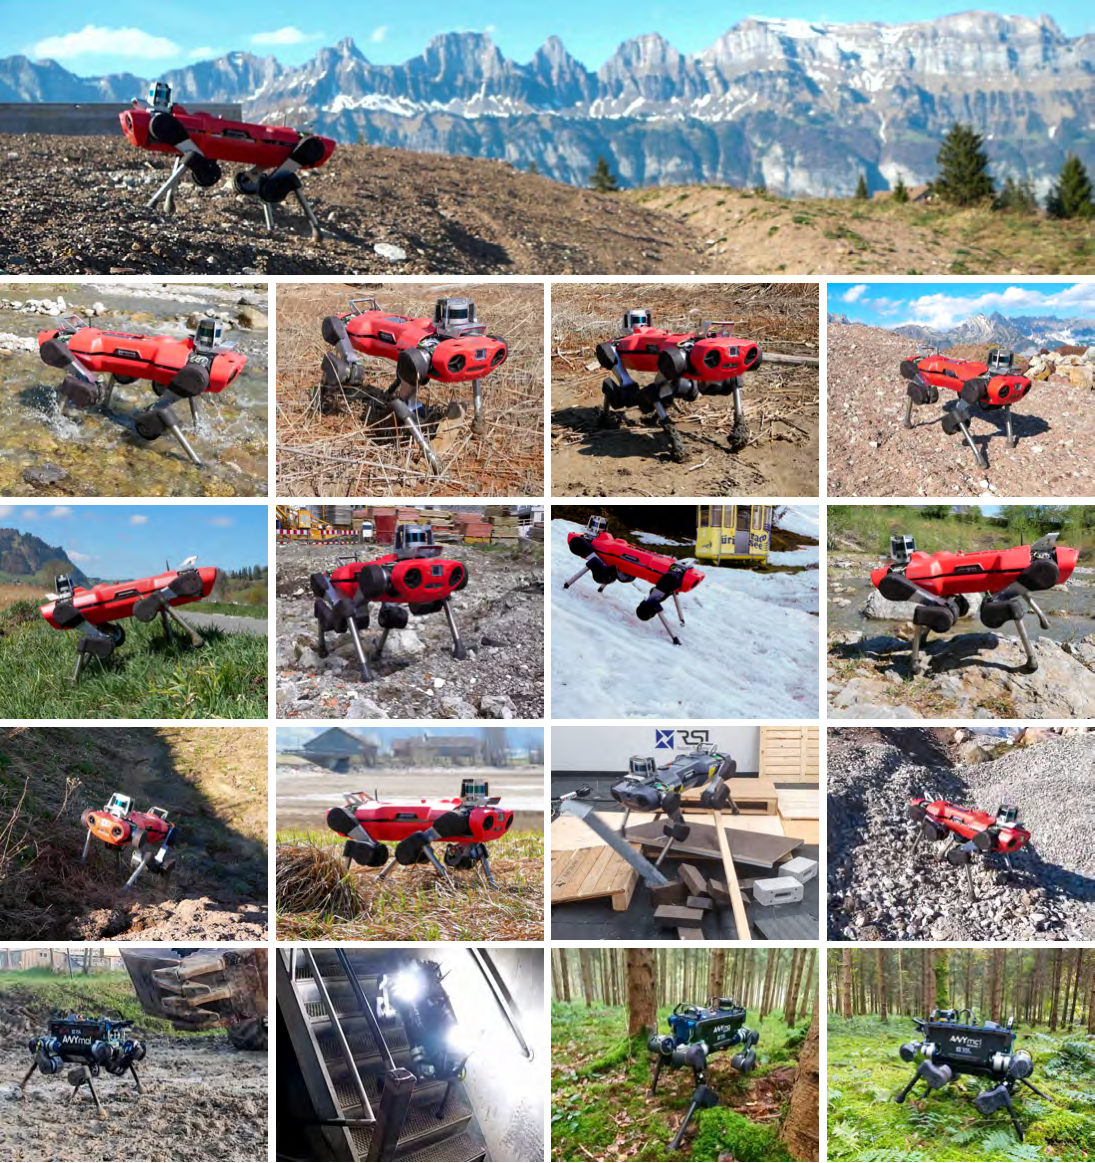
\includegraphics[width=\textwidth]{img/figure1.pdf}
    \caption{\textbf{本文提出的运动控制器在多种挑战性环境中的部署。}}
    \label{fig:1}
\end{figure*}

\section{引言}
腿足运动（Legged Locomotion）能够极大地扩展机器人学的应用范围。
地球上大部分干燥陆地仍然是轮式和履带式机器无法通行的，这些机器在挑战性地形上的稳定性会受到严重影响。
而四足动物则可以到达地球上一些最偏远的区域。
它们能够在运动学可达范围内选择安全的落足点，并快速改变运动学状态以应对环境。腿足机器人有潜力穿越与动物对手相同的任何地形。

迄今为止，尚无已发表的工作展示了如图~\ref{fig:1}所示在多样且具有挑战性的自然环境中的动态运动。
这些环境具有高度不规则的轮廓、可变形地形、光滑表面以及地面障碍物。
在此类条件下，现有已发表的控制器会出现频繁的足部打滑（Foot Slippage）、失去平衡，并最终导致灾难性故障。
由于无法获取地形物理特性的真实信息，这一挑战更加严峻。
摄像头和LiDAR等外部感知传感器无法可靠地测量摩擦系数和刚度等物理特性，会因植被、雪和水等障碍物而受阻，并且可能无法达到覆盖范围和时域分辨率来捕捉机器人自身引起的变化，例如机器人脚下松散地面的崩塌。
在这些条件下，机器人必须关键地依赖本体感知——以高时间分辨率感知自身身体构型。
面对意外事件（如意外地面接触、地形变形和足部打滑），控制器必须快速生成满足多个目标的全身轨迹：保持平衡、避免自碰撞、抵抗外部干扰以及运动。虽然动物本能地解决了这一复杂控制问题，但在机器人学中仍然是一个开放的挑战。

在不平地形上实现腿足运动的传统方法产生了日益复杂的控制架构。许多方法依赖于精心设计的状态机来协调运动基元和反射控制器的执行~\cite{jenelten2019dynamic,bledt2018contact,focchi2020heuristic,Reher2019,gong2019feedback}。为了触发状态之间的转换或反射的执行，许多系统显式估计地面接触和打滑等状态~\cite{hwangbo2016probabilistic,camurri2017probabilistic,focchi2018slip}。这种估计通常基于经验调整的阈值，在泥地、雪地或植被等未建模因素存在时可能变得不稳定。其他系统在足部使用接触传感器，这在现场条件下可能变得不可靠~\cite{Bloesch2013,gehring2015dynamic,hartley2018legged}。总体而言，用于粗糙地形的腿足运动传统系统随着考虑更多场景而日益复杂，开发和维护工作量极大，且仍然容易受到边界情况的影响。

无模型强化学习（Reinforcement Learning, RL）最近已成为开发腿足运动技能的一种替代方法~\cite{hwangbo2019learning,haarnoja2018learning,xie2019iterative}。
RL的思想是通过优化控制器来最大化给定的奖励函数（Reward Function）。优化过程基于执行控制器本身所获取的数据，并随着经验积累而改善。RL已被用于简化运动控制器的设计、自动化设计过程的某些部分，以及学习先前方法无法设计的行为~\cite{hwangbo2019learning,lee2019robust,haarnoja2018learning,xie2019iterative}。

然而，RL在腿足运动中的应用在很大程度上仍局限于实验室环境和条件。本文的先前工作展示了运动与恢复行为的端到端学习——但仅限于实验室的平坦地面~\cite{hwangbo2019learning}。其他工作也开发了用于腿足运动的RL技术，但同样主要关注实验室环境中的平坦或适度纹理表面~\cite{tan2018sim,haarnoja2018learning,xie2019iterative,yang2019data,ha2020learning,Peng2020}。

本文提出了一种在挑战性地形上进行盲态四足运动的极其鲁棒的控制器。该控制器仅使用来自关节编码器（Joint Encoder）和惯性测量单元（Inertial Measurement Unit, IMU）的本体感知测量值，这些是腿足机器上最耐用、最可靠的传感器。控制器的工作情况如图~\ref{fig:1}和\href{https://youtu.be/9j2a1oAHDL8}{Movie~1}所示。该控制器用于驱动两代ANYmal四足机器人~\cite{hutter2016anymal}在各种条件下运行，这些条件超越了先前已发表的腿足机器人工作所能达到的范围。该控制器可靠地穿越泥地、沙地、碎石、茂密植被、雪地、流水以及其他多种越野地形。相同的控制器还被用于本文参加DARPA地下挑战赛城市赛段的比赛。
在所有部署中，同代机器人在所有条件下均使用完全相同的控制器。
无需为适应不同环境进行任何调整。

与先前许多将无模型RL应用于腿足运动的工作一样，本文在仿真（Simulation）中训练控制器~\cite{hwangbo2019learning,tan2018sim,xie2019iterative}。先前的工作已确立了一系列将腿足运动控制器从仿真成功迁移到物理机器的实践方法。其中之一是对物理系统（包括执行器（Actuator））进行逼真建模~\cite{hwangbo2019learning}。另一项是对仿真与真实世界之间变化的物理参数进行随机化，使控制器对物理部署中可能遇到的一系列条件具有鲁棒性，而无需事先精确建模这些条件~\cite{peng2018sim}。

本文也采用了这些思想，但发现它们不足以在粗糙地形上实现鲁棒的运动。因此，本文引入并验证了对于实现所述技能至关重要的若干额外要素。第一个是不同的策略（Policy）架构。与先前工作中常见的基于当前机器人状态快照的多层感知机（Multi-Layer Perceptron, MLP）不同，本文使用序列模型，具体而言是时序卷积网络（Temporal Convolutional Network, TCN）~\cite{bai2018empirical}，该网络基于本体感知状态的扩展历史生成驱动指令。本文不采用显式的接触和打滑估计模块（已知在挑战性情况下不可靠）；相反，TCN根据需要从本体感知历史中隐式推理接触和打滑事件。

第二个实现所述结果的重要思想是特权学习（Privileged Learning）~\cite{chenlearning}。本文发现直接通过RL训练粗糙地形运动策略并不成功：监督信号稀疏，所提出的网络无法在合理时间预算内学会运动。相反，本文将训练过程分解为两个阶段。首先，训练一个能够访问特权信息（即地形的真实状态以及机器人与地形的接触信息）的教师策略（Teacher Policy）。特权信息使策略能够快速达到高性能。然后，利用这个特权教师来指导仅使用真实机器人上可用传感器的纯本体感知学生策略（Student Policy）的学习。这种特权学习协议依赖于仿真实现，但最终的本体感知策略并不局限于仿真，可直接部署在物理机器上。

第三个对实现所展示的鲁棒性水平至关重要的思想是自动课程（Curriculum），它根据控制器在训练过程不同阶段的性能自适应地生成地形。本质上，地形被合成为控制器能够穿越的形式，同时使其变得更加鲁棒。本文评估参数化地形的可穿越性，并使用粒子滤波来维护中等难度地形参数的分布~\cite{brant2017minimal,wang2019paired}，该分布随着神经网络的学习而自适应调整。训练条件逐渐变得更加具有挑战性，最终产生了一个兼具敏捷性和前所未有的韧性的全向运动控制器。

最终成果是一个比现有文献中任何对手都更加鲁棒的腿足运动控制器。值得注意的是，该控制器在零样本泛化（Zero-Shot Generalization）设置中始终有效。也就是说，当在训练中从未经历过的条件下测试时，它仍然保持鲁棒性。本文的仿真训练仅使用刚性地形和少量程序化生成的地形轮廓（如丘陵和台阶）。然而，当部署在物理四足机器人上时，控制器成功应对了可变形地形（泥地、苔藓、雪地）、动态落足点（在杂乱的室内环境中踩上滚动的木板，或现场中的碎片）以及地面障碍物（如茂密植被、碎石和汹涌水流）。本文的方法和结果为腿足机器人学开辟了新前沿，并表明物理世界的非凡复杂性可以通过无需脆弱且费力的建模或危险且昂贵的现场试错来驯服。

\section{结果}
\begin{figure}
    \centering
  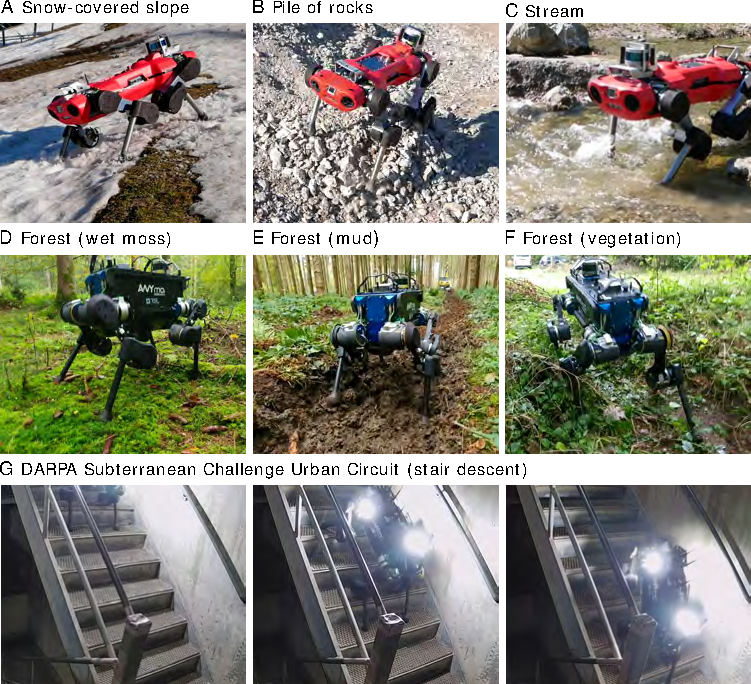
\includegraphics[width=\linewidth]{img/figure2.pdf}
    \caption{\textbf{若干特定部署场景。}
    (\textbf{A-F}) 对光滑和变形地形的零样本泛化。
    (\textbf{G}) DARPA地下挑战赛期间的陡峭下坡。台阶高度为18 cm，坡度约为$\sim 45^{\circ}$。
      }\label{fig:2}
\end{figure}
\begin{figure*}
    \centering
     \makebox[\textwidth][c]{
    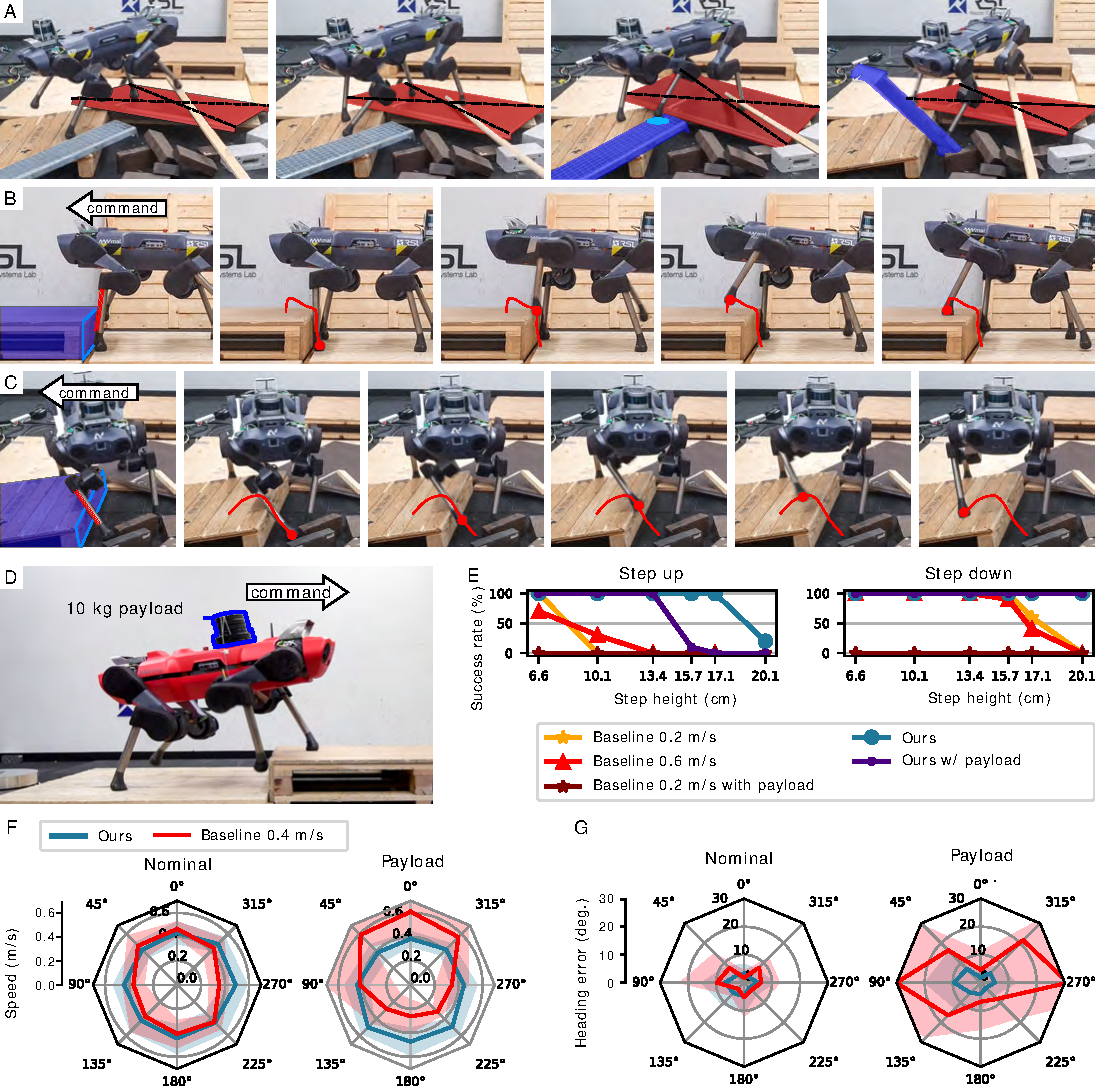
\includegraphics[width=\textwidth]{img/figure3.pdf}
    }
    \caption{\textbf{室内环境评估。}
    (\textbf{A}) 在不稳定碎片上的运动。机器人踩上松动的木板（红色和蓝色高亮），这些木板在机器人脚下发生移动。
    (\textbf{B}) 策略表现出足部卡陷反射，并越过\unit[16.8]{cm}高的台阶。
    (\textbf{C}) 策略学会无论接触位置如何均能恰当处理障碍物。图中展示了在摆动相期间小腿中部遇到障碍物时的反应。
    (\textbf{D}) 台阶和负载的受控实验。本文控制器和基线方法~\cite{bellicoso2018dynamic,jenelten2019dynamic}被命令在有和没有\unit[10]{kg}负载的情况下翻越台阶。
    (\textbf{E}) 不同台阶高度的成功率。每种条件评估10次试验的成功率。
    (\textbf{F}) 平地上不同指令方向的平均线速度。\unit[0]{$^\circ$}指向机器人前方。阴影区域表示\unit[95]{\%}置信区间。(\textbf{G}) 平地上不同指令方向的平均航向误差。阴影区域表示\unit[95]{\%}置信区间。
    }\label{fig:3}
\end{figure*}

\href{https://youtu.be/9j2a1oAHDL8}{Movie~1}总结了本文工作的结果。
本文将训练好的运动控制器部署在两代ANYmal机器人上：ANYmal-B（图~\ref{fig:2}D-G）和ANYmal-C（图~\ref{fig:2}A-C和图~\ref{fig:3}）。
这些机器人具有不同的运动学特性、惯性和执行器。

\subsection*{自然环境}

本文提出的控制器已部署在多种自然环境中，如图~\ref{fig:1}和\href{https://youtu.be/9j2a1oAHDL8}{Movie~1}及\href{https://youtu.be/txjqn8h6pjU}{Movie~S1}所示。这些环境包括陡峭的山间小径、流淌的溪流、泥地、茂密植被、松散碎石、积雪覆盖的山丘以及潮湿的森林。
图~\ref{fig:2}A-F进一步突出展示了若干具体场景。这些环境具有策略在训练中未曾经历的特性。地形可能变形和崩塌，材料属性在表面上具有显著变化。由于植被、碎石和粘性泥地，机器人的腿部频繁受到干扰。
使用摄像头或LiDAR的现有地形估计流程~\cite{fankhauser2014robot}在雪地（图~\ref{fig:2}A）、水域（图~\ref{fig:2}C）或茂密植被（图~\ref{fig:2}F）中会失败。本文控制器不依赖外部感知，因此不受此类故障的影响。控制器基于本体感知观测历史学习全向运动，并且在具有训练中从未经历过特性的地形上进行零样本部署时具有鲁棒性。

本文将所提出的控制器与最先进的基线方法~\cite{bellicoso2018dynamic,jenelten2019dynamic}在森林环境中进行了比较。基线方法能够穿越平坦且无障碍的区域，但在遇到松散树枝、茂密植被和泥地时频繁失败，如\href{https://youtu.be/txjqn8h6pjU}{Movie~S1}所示。本文控制器在这些实验中从未失败。

\begin{table}
\centering
 \begin{tabular}{|c|c|c|c|c|}
\hline
\multirow{2}{*}{指标} & \multirow{2}{*}{控制器} &  \multicolumn{3}{|c|}{地形} \\ \cline{3-5}
  & & 苔藓 & 泥地 & 植被 \\ \hline
  \multirow{2}{*}{ \parbox{2cm}{\centering 平均速度 \\ ($m/s$)}} &
本文方法 & \textbf{0.452} & \textbf{0.338} & \textbf{0.248} \\ \cline{2-5}
& 基线方法 & 0.199 & 0.197 & --  \\ \hline
  \multirow{2}{*}{ \parbox{2cm}{\centering 平均 \\ 机械 \\ COT}} &
本文方法 & \textbf{0.423} & \textbf{0.692} & \textbf{1.23} \\ \cline{2-5}
& 基线方法 & 0.625 & 0.931& --  \\ \hline
 \end{tabular}
\caption{\textbf{自然环境中运动性能对比。}机械COT使用执行器输出的正机械功率计算。}
\label{tab:1}
\end{table}


本文对提出的控制器与基线方法在三种条件下进行了定量评估：苔藓、泥地和植被（图~\ref{fig:2}D-F）。本文测量了运动速度和能效。结果报告在表~\ref{tab:1}中。本文提出的控制器在所有条件下都实现了更高的运动速度。
本文计算了无量纲的运输成本（Cost of Transport, COT）来比较不同速度范围内控制器的效率。
本文将机械COT定义为$\sum_{\text{12 actuators}}{[\tau \dot{\theta}]^{+}}  / (mgv)$。$\tau$表示关节力矩，$\dot{\theta}$表示关节速度，$mg$表示总重量，$v$表示运动速度。
该指标表示执行器在单位重量和单位运动速度下输出的正机械功率~\cite{collins2005efficient}。
如表~\ref{tab:1}所示，本文提出的控制器能效更高，COT低于基线方法。

表~\ref{tab:1}中报告的定量评估低估了两者之间的差异，因为它仅测量基线方法成功运动时的速度和能效。
基线方法的灾难性故障未被纳入这些测量：当基线方法失败时，由人类操作员在更稳定的构型下重置。因茂密植被等因素导致的基线控制器灾难性故障如\href{https://youtu.be/txjqn8h6pjU}{Movie~S1}所示。本文控制器未出现此类故障。

\subsection*{DARPA地下挑战赛}
本文控制器被CERBERUS团队用于DARPA地下挑战赛城市赛段（图~\ref{fig:2}G）。它取代了该团队过去使用的基于模型的控制器~\cite{bellicoso2018dynamic,jenelten2019dynamic}。
比赛的目标是开发能够快速测绘、导航和搜索复杂地下环境（包括隧道、城市地下空间和洞穴网络）的机器人系统。
比赛期间不允许人类操作员物理协助机器人；仅允许远程操作。
因此，运动控制器需要在长时间任务中无故障运行。
据本文所知，这是通过无模型RL训练的腿足运动控制器在此类竞争性现场部署中的首次使用。

本文提出的控制器在四次各60分钟的任务中驱动了两台ANYmal-B机器人。
在整个比赛中，控制器表现出零故障率。
比赛期间其中一台机器人翻越的陡峭楼梯如图~\ref{fig:2}G所示。

\subsection*{室内实验}
本文进一步在布满松散碎石的室内环境中评估了所提出控制器的鲁棒性，如图~\ref{fig:3}A所示。
支撑面不稳定，机器人的足部频繁打滑。
这样的条件可在灾难现场和建筑工地中找到，而腿足机器人预计将在未来运行于这些环境中。

结果如图~\ref{fig:3}A和\href{https://youtu.be/Xnn4sVSpSh0}{Movie~S2}所示。机器人全向移动穿越该区域。本文提出的控制器能够在移动的支撑面上稳定运动。
这种鲁棒性水平超越了先前ANYmal机器人的控制器所能达到的范围~\cite{bellicoso2018dynamic,jenelten2019dynamic}，与最先进水平相当~\cite{bledt2018contact,vision60blind}。

学习到的控制器展现出足部卡陷反射，如图~\ref{fig:3}B和\href{https://youtu.be/tPixnjLbTvE}{Movie~S3}所示。
策略仅从本体感知观测中识别足部卡陷，并抬起足部越过障碍物。
%than the usual foot clearance (i.e., maximum height of a swing foot).
此类反射在训练过程中未经任何明确指定：它们是自适应发展而来的。这使本文方法区别于传统的控制器设计方法，后者明确构建此类反射并通过高层状态机协调其执行~\cite{jenelten2019dynamic,focchi2020heuristic}。
图~\ref{fig:3}B中所示的台阶高度为\unit[16.8]{cm}，高于平地上正常行走时腿部的离地高度。
平地上的最大离地高度分别为LF腿和RF腿的\unit[12.9]{cm}和\unit[13.6]{cm}\footnote{本文用L、R、F、H分别表示左、右、前、后，以紧凑地指代腿部。例如，'LF腿'指左前腿。}，在足部卡陷情况下分别增加到\unit[22.5]{cm}和\unit[18.5]{cm}。
本文控制器还学会了在上台阶时调整后腿轨迹。平地上LH和RH腿的最大离地高度分别为\unit[13.5]{cm}和\unit[9.06]{cm}，当前腿越过台阶时增加到\unit[16.6]{cm}和\unit[15.9]{cm}。进一步分析见材料与方法部分。
还需注意，本文控制器学习到的反射更加通用，不局限于特定的接触事件。图~\ref{fig:3}C展示了控制器对摆动相中小腿中部碰撞的响应。在此情况下，卡陷事件并非由足部接触触发，使用足部接触事件作为触发器的脚本化控制器无法正确处理此情况。而本文控制器则将本体感知流作为一个整体进行分析，且训练过程中未对可能的接触位置做出假设。因此，它可以学会对任何影响机器人身体构型的障碍物和干扰做出反应。

%\subsection*{Controlled comparison with the existing method}
现在本文专注于在受控设置中将所提出的方法与基线方法~\cite{bellicoso2018dynamic,jenelten2019dynamic}进行比较。
本文首先在单一台阶的诊断性设置中比较控制器的鲁棒性，如图~\ref{fig:3}D所示。
在每次试验中，机器人被命令直行翻越台阶，持续\unit[10]{s}。如果机器人的前后腿均成功翻越台阶，则试验成功。本文对每种台阶高度进行10次试验，并计算成功率。
由于基线控制器以基座的期望线速度作为输入，本文指令的前进速度为\unit[0.2]{m/s}和\unit[0.6]{m/s}。\unit[0.6]{m/s}是基线控制器的最大速度。
成功率如图~\ref{fig:3}E所示。本文提出的控制器在上台阶和下台阶方面均优于基线方法。
基线方法对足部卡陷表现出高敏感性，这经常导致摔倒，如\href{https://youtu.be/tPixnjLbTvE}{Movie~S3}所示。

本文还测试了存在显著模型失配时控制器的性能。本文添加了一个\unit[10]{kg}的负载，如图~\ref{fig:3}D和\href{https://youtu.be/3Nr47MXCFO0}{Movie~S4}所示。该负载占机器人总重量的\unit[22.7]{\%}，且在训练过程中从未模拟过。如图~\ref{fig:3}E所示，尽管存在模型失配，本文提出的控制器仍能翻越高达\unit[13.4]{cm}的台阶。基线方法在负载下无法以任何指令速度翻越任何台阶。

本文随后评估了控制器在平坦地面上带负载的跟踪性能。
本文向每个控制器指令8个方向，并测量运动速度和跟踪误差。
基线控制器的目标速度固定为\unit[0.4]{m/s}，与本文提出控制器的工作速度相近。
在图~\ref{fig:3}F中，本文展示了控制器的速度分布。本文控制器在所有方向上的运动速度约为\unit[0.4]{m/s}，并在带负载时表现相似。
另一方面，基线方法的运动速度随方向变化，可从各向异性的速度分布看出，且带负载时速度分布显著偏离中心。
图~\ref{fig:3}G展示了每个指令方向下控制器的航向误差。航向误差是指令速度与机器人基座速度之间的夹角。本文提出的控制器的航向误差始终小于基线方法，无论有无负载。
基线方法在横向方向上的误差达到$\sim$\unit[30]{$^\circ$}，并且当指令速度为(\unit[0.6]{m/s})时基线方法失败，如\href{https://youtu.be/3Nr47MXCFO0}{Movie~S4}所示。
相比之下，本文提出的控制器的平均航向误差无论有无负载均保持在\unit[10]{$^\circ$}以内。本文得出结论，提出的控制器对模型失配具有更强的鲁棒性。

接下来本文测试对足部打滑的鲁棒性。
为引入打滑，本文使用了湿润的白板~\cite{jenelten2019dynamic}。
结果如\href{https://youtu.be/aMPwB3t4idU}{Movie~S5}所示。
基线方法迅速失去平衡，剧烈摆动腿部并摔倒。相比之下，本文提出的控制器适应了光滑地形并成功地在指令方向上运动。

\section{讨论}
本文提出的结果显著推进了腿足机器人学的已发表最先进水平。除了结果本身，本文提出的方法可以具有广泛的应用。在本文工作之前，可能存在一种假设，即仿真训练的固有局限性在于仿真环境无法代表物理世界的复杂性。当前技术在模拟柔性接触、打滑以及可变形和崩塌地形方面能力严重受限。因此，泥地、雪地、茂密植被、汹涌水流等现象超出了机器人仿真框架的能力范围~\cite{hwangbo2018per,coumans2013bullet,smith2005open}。无模型RL算法的样本复杂性（通常需要数百万时间步进行训练）进一步加剧了挑战，排除了对可能需要每时间步数秒计算的框架的依赖。

本文工作表明，模拟物理世界的惊人多样性可能并非必要。本文的训练环境仅包含刚性地形，没有柔性或地面障碍物（如植被）。然而，在此环境中训练的控制器成功应对了部署时遇到的各种现场条件。

本文看到若干局限性和未来工作的机会。首先，本文提出的控制器仅表现出一种步态（Gait）——踱步步态（Trot）。这比自然界中四足动物发现的步态模式范围更窄~\cite{Alexander2003}。步态模式部分受限于机器人的运动学和动力学，但ANYmal机器人在物理上能够实现多种步态~\cite{bellicoso2018dynamic}。本文假设，强调多样性的训练协议和目标可以引出这些步态。

其次，本文提出的控制器仅依赖本体感知。这是一个显著优势，因为控制器对传感器套件的要求很少，并且不会在外部感知失效时受到影响。事实上，现有工作已经主张盲态（本体感知）控制器应构成腿足运动栈的基础~\cite{focchi2020heuristic}。然而，盲态运动本质上是有局限性的。如果机器被指令走下悬崖，它就会照做。即使在不那么极端的条件下，机器人的步态也相当保守，因为它必须通过身体感知环境来运动。未来工作的一个重要机会是将本文提出的方法作为起点，开发混合本体感知-外部感知控制器——如同许多动物一样——即使在视觉和其他外部感官受到干扰时也能运动，但在有外部感知数据时加以利用。这将使腿足机器能够自主穿越具有悬崖等致命元素的环境，并在更安全的条件下提高速度和能效。

更广泛地说，本文提出的结果加速了腿足机器在轮式和履带式机器人无法到达、对人类而言危险或不可及的环境中的部署，同时本文提出的方法为在仿真中训练复杂机器人系统并将其部署于物理世界的全部丰富性和复杂性中开辟了新前沿。

\section{材料与方法}

\begin{figure*}
    \centering
    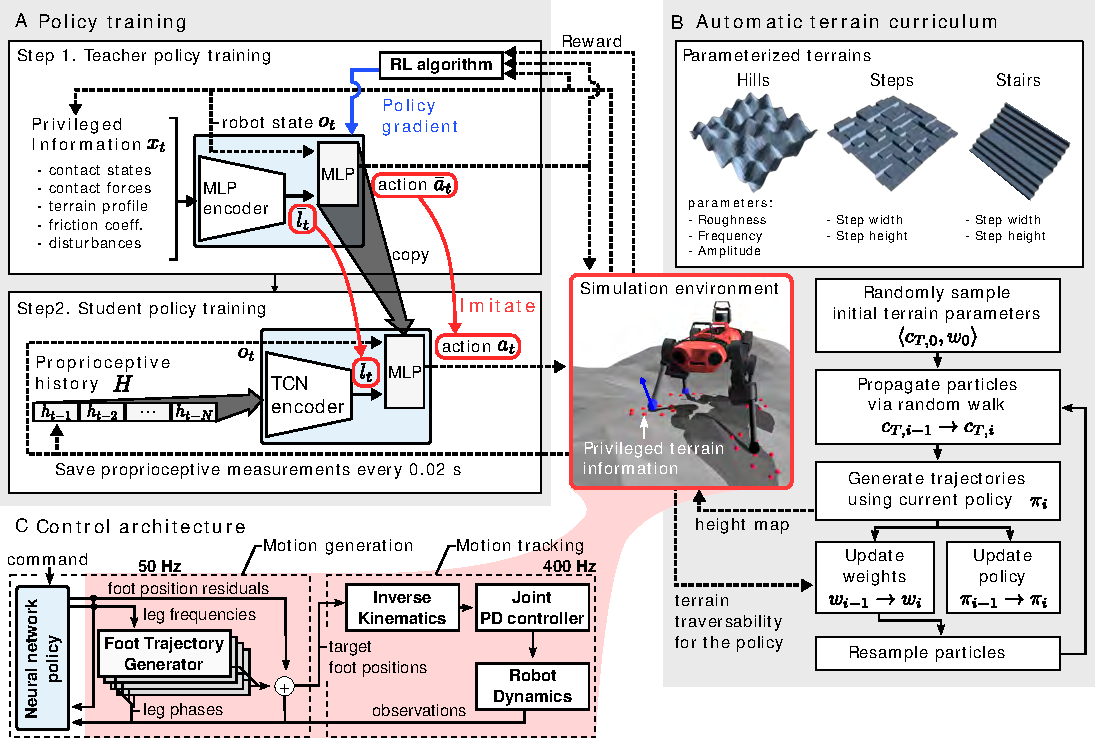
\includegraphics[width=\textwidth]{img/figure4.pdf}
    \caption{\textbf{本文方法概览。} (\textbf{A})~两阶段训练过程。首先，在仿真中使用RL训练教师策略（Teacher Policy）。教师策略可以访问真实世界中无法获得的特权信息（Privileged Information）。
    然后，纯本体感知学生策略（Student Policy）通过模仿教师来学习。学生策略基于本体感知传感输入流进行决策，不使用特权信息。
    (\textbf{B})~自适应地形课程（Adaptive Terrain Curriculum）在训练过程中合成适当难度等级的地形。使用粒子滤波来维护一组具有挑战性但策略可穿越的地形参数分布。
    (\textbf{C})~运动控制器的架构。学习到的本体感知策略通过运动学残差调节运动基元。关节PD控制器的经验模型便于在物理机器上部署。
    }
    \label{fig:4}
\end{figure*}

\subsection{概述}

本文提出的控制器的主要目标是根据指令在粗糙地形上运动。
指令由人类操作员或高层导航控制器给出。
在本文的公式中，与许多现有工作~\cite{hwangbo2019learning,tan2018sim,xie2019iterative}关注跟踪目标基座速度不同，仅方向（$^B_{IB} \hat{v}_T$）被提供给控制器。
原因在于，在挑战性地形上目标速度的可行范围通常不明确。例如，机器人下坡比上坡可以走得更快。

指令向量定义为$\langle (^{B}_{IB}\hat{v}_{T})_{xy}, (\hat{\omega}_{T})_{z} \rangle$。
第一部分是基座坐标系中的目标水平方向$(^{B}_{IB}\hat{v}_{T})_{xy} \coloneqq \langle \cos(\psi_T), \sin(\psi_T) \rangle$，其中$\psi_T$是基座坐标系中指令方向的偏航角。停止指令定义为$\langle0.0, 0.0\rangle$。第二部分是转向方向$(\hat{\omega}_{T})_{z} \in \{-1, 0, 1 \}$。1表示绕基座$z$轴逆时针旋转。

本文方法的概览如图~\ref{fig:4}所示。
本文采用受learning by cheating~\cite{chenlearning}启发的特权学习策略（图~\ref{fig:4}A）。
首先训练一个能够访问地形特权信息的教师策略。然后将该教师策略蒸馏到不依赖特权信息的纯本体感知学生策略中。特权教师策略局限于仿真，但学生策略部署在物理机器上。本文方法与Chen等人~\cite{chenlearning}的方法的一个区别在于，本文不依赖专家演示来训练特权策略；相反，教师策略通过RL训练。

特权教师模型基于多层感知机（Multi-Layer Perceptrons, MLPs），接收机器人当前状态、地形属性以及机器人与地形接触的信息。模型计算表示当前状态的潜在嵌入$\bar{l}_t$和动作$\bar{a}_t$。
训练目标奖励在指定方向上的运动。

教师策略训练完成后，用于监督纯本体感知学生策略。学生模型是时序卷积网络（Temporal Convolutional Network, TCN）~\cite{bai2018empirical}，接收$N$个本体感知观测序列作为输入。学生策略通过模仿进行训练。教师策略计算的向量$\bar{l}_t$和$\bar{a}_t$用于监督学生。如图~\ref{fig:4}A所示。

训练在仿真中程序化生成的地形上进行。地形自适应地合成，以根据训练策略在任何给定时间的技能水平促进学习。本文定义了地形的可穿越性度量，并开发了一种基于采样的方法，在训练过程中选择适当难度的地形。本文使用粒子滤波来维护适当的地形参数分布。如图~\ref{fig:4}B所示。
地形课程在教师和学生训练过程中均被应用。

本文的控制架构如图~\ref{fig:4}C所示。
本文采用策略调节轨迹生成器（Policies Modulating Trajectory Generators, PMTG）架构~\cite{iscen2018policies}来提供运动生成的先验。
神经网络策略通过合成残差位置指令来调节腿部相位和运动基元。

仿真使用机器人关节PD控制器的学习动力学模型~\cite{hwangbo2019learning}。这有助于策略从仿真迁移到现实。在仿真中训练后，本体感知控制器直接部署在物理腿足机器上，无需微调。

\subsection*{运动合成}

现在本文详细阐述图~\ref{fig:4}C中所示的控制架构。它分为运动生成和跟踪两部分。
本文控制器的输入包括指令向量以及一系列本体感知测量值，包括基座速度、方向和关节状态。
控制器不使用任何外部感知输入（例如，无触觉传感器、摄像头或深度传感器）。输入也不包含任何人工设计的特征，如足部接触状态或估计的地形几何形状。
控制器输出关节位置目标。

本文的运动生成策略基于周期性腿部相位。
先前的工作通常利用预定义的足部接触时间表~\cite{barasuol2013reactive,bledt2018contact,bellicoso2018dynamic}。
本文为每条腿定义一个周期性相位变量$\phi_{i} \in [0.0, 2\pi)$，其中$\phi \in [0.0, \pi)$表示接触相（Stance Phase），$\phi \in [\pi, 2\pi)$表示摆动相（Swing Phase）。
在每个时间步$t$，$\phi_i = (\phi_{i,0} + (f_0 + f_i)t ) \pmod{2 \pi}$，其中$\phi_{i,0}$是初始相位，$f_0$是公共基频，$f_i$是第$i$条腿的频率偏移。本文希望当$f_0+f_i \neq 0$时腿部展现周期性运动，并在接触相中与地面接触。
本文将$f_0$设为\unit[1.25]{Hz}，这是先前为踱步步态开发的传统控制器所使用的值~\cite{bellicoso2018dynamic}。

目标足部位置（运动生成块的输出）定义在足部水平坐标系（Horizontal Frame）~\cite{barasuol2013reactive} $H_{i}, i\in \{1,2,3,4 \}$中。
$H_i$是连接在第$i$条腿髋关节下方的参考坐标系。
距离等于腿的标称可达范围。
该坐标系的$z$轴（$^{H_i}z$）平行于$e_g$，$^{H_i}x$是基座$x$轴（$^{B}x$）在水平面上的投影，即该坐标系与机器人具有相同的偏航角。
$H_i$的横滚角和俯仰角与基座解耦。
这种运动学技巧减少了基座姿态对足部运动的影响~\cite{barasuol2013reactive}，从而稳定了训练。
在$H_i$中定义输出减少了策略训练初期的过早终止，此时基座运动由于随机动作而不稳定。
另一个好处是，本文可以在策略训练期间将随机策略的动作分布在横向和垂直方向上进行分解。本文在横向方向施加更大的噪声，以促进沿地面的探索。

本文使用PMTG架构~\cite{iscen2018policies}将神经网络集成到控制器中。
本文的实现包含四个相同的足部轨迹生成器（Foot Trajectory Generator, FTG）和一个神经网络策略。
FTG是函数$F(\phi): [0.0, 2\pi) \rightarrow \mathbb{R}^3$，输出每条腿的目标足部位置。当$f_i$非零时，FTG驱动垂直迈步运动。$F(\phi)$的定义见补充材料第S3节。

策略输出$f_i$和目标足部位置残差（$\Delta {r}_{f_i,T}$），第$i$个足部的目标位置为$r_{f_i,T} \coloneqq F(\phi_i) + \Delta{r}_{f_i,T}$。

跟踪控制使用解析逆运动学（Inverse Kinematics, IK）和关节位置控制完成。
每个在$H_i$中定义的目标足部位置首先转换到机器人基座坐标系，然后使用解析IK计算关节位置目标。
关节位置目标随后由关节位置PD控制器跟踪。
使用解析IK的主要原因是最大化计算效率，并重用现有位置控制执行器模型~\cite{hwangbo2016probabilistic,lee2019robust}以进行仿真到真实（Sim-to-Real）迁移。

\subsection*{教师策略}

本文将控制问题形式化为马尔可夫决策过程（Markov Decision Process, MDP）。
MDP是用于建模离散时间控制过程的数学框架，其中状态演化和结果部分随机。
MDP由状态空间$\mathcal{S}$、动作空间$\mathcal{A}$、标量奖励函数$\mathcal{R}(s_t, s_{t+1})$以及转移概率$P(s_{t+1} | s_t, a_t)$定义。
学习智能体根据其策略$\pi(a_t|s_t)$选择动作$a_t$，并从环境中获得奖励$r_t$。
RL框架的目标是找到最优策略$\pi^*$，最大化无限时间范围内的折扣奖励总和。

假设环境对教师完全可观测，本文将运动控制建模为MDP，并使用现成的RL方法~\cite{schulman2015trust}求解。本节中，本文提供教师训练的MDP，由状态空间、动作空间、转移概率和奖励函数的元组定义。

状态定义为$s_t \coloneqq \langle o_t, x_t \rangle$，其中$o_t$是从机器人可获得的状态测量向量，$x_t$是通常在真实世界中无法获得的特权信息。详细定义见表S4。
$o_t$包含指令、方向、基座扭转、关节位置和速度、$\phi_i$s、$f_i$s以及先前的目标足部位置。$o_t$中还包含在\unit[-0.01]{s}和\unit[-0.02]{s}处测量的关节位置误差和速度，这与关节级PD控制器的学习模型输入相同。
这些信息允许策略利用执行器动力学~\cite{hwangbo2019learning}。
为了编码腿部相位，本文使用$\langle \cos(\phi), \sin(\phi) \rangle$代替$\phi$，这是一种光滑且唯一的角表示。
先前的目标足部位置也被反馈给策略，用于计算下文所述的目标平滑度奖励。
当学生控制器部署时，$o_t$中的量被替换为本体感知传感器的读数，基座速度和方向由状态估计器提供~\cite{bloesch2013state}。
$x_t$包含直接从物理引擎获得的无噪声信息。
$x_t$主要包含与足地交互相关的信息，如地形轮廓、足部接触状态和力、摩擦系数以及训练期间施加的外部干扰力。具体而言，本文使用每个足部周围9个扫描点的高程来表示地形轮廓，这些点沿半径为\unit[10]{cm}的圆对称布置（如图~\ref{fig:4}所示）。

动作（$\bar{a}_t$）是16维向量，包含腿部频率和足部位置残差。

奖励函数定义为：RL智能体若更快朝目标前进，则获得更高奖励。奖励函数的详细说明见补充材料第S4节。

策略网络由图~\ref{fig:4}A所示的两个MLP块构建。
MLP编码器将$x_t$嵌入到潜在向量$\bar{l}_t$中。
指令和机器人状态不包含在$x_t$中，因此$\bar{l}_t$仅包含地形和接触相关的特征。
本文假设$\bar{l}_t$驱动自适应行为，例如根据地形轮廓改变离地高度。
然后$\bar{l}_t$和$o_t$被提供给后续的MLP层以计算动作。

信任区域策略优化（Trust Region Policy Optimization, TRPO）~\cite{schulman2015trust}算法用于训练。
所使用的超参数见表S7。

\subsection*{学生策略}

本体感知学生策略只能访问$o_t$。
这里的一个关键假设是，潜在特征$\bar{l}_t$可以从本体感知观测的时间序列$h_t$中（部分）恢复，其中$h_t$定义为$ h_t \coloneqq o_t \setminus \{f_o, \text{joint history}, \text{previous foot position targets} \}$。

学生策略使用时序卷积网络（Temporal Convolutional Network, TCN）~\cite{bai2018empirical}编码器。
TCN编码器的输入是$H = \{h_{t-1}, ..., h_{t-N-1}\}$，其中$N$是历史长度。
编码器是全卷积的，由三个膨胀因果卷积层组成，其间穿插降维的步长卷积层。
架构详见表S5和S6。

本文使用TCN架构，因为它允许透明控制输入历史长度、能够容纳长历史记录，并且已知对超参数设置具有鲁棒性~\cite{bai2018empirical}。与循环神经网络架构的比较见补充材料第S8节。

学生策略通过监督学习进行训练。损失函数定义为
\begin{equation}
    \mathcal{L} \coloneqq (\bar{a_t}(o_t, x_t) - a_t(o_t, H))^2 +  (\bar{l_t}(o_t, x_t) - l_t(H))^2.
\label{eq:student}\end{equation}
带有横线（$\bar{\cdot}$）的量表示教师生成的目标值。
本文采用数据集聚合策略（Dataset Aggregation, DAgger）~\cite{ross2011reduction}。具体而言，训练数据通过学生策略的轨迹展开生成。对于每个访问过的状态，教师策略计算其嵌入向量和动作向量（$\bar{\cdot}$）。教师策略的这些输出用作对应状态的监督信号。
所使用的超参数见表S8。

\subsection*{自适应地形课程}

本文方法受RL智能体自动课程学习（Automatic Curriculum Learning, ACL）的启发~\cite{wang2019paired,florensa2018automatic}。配对开放式开拓者（Paired Open-Ended Trailblazer, POET）方法~\cite{wang2019paired}为二维双足智能体生成多样化的参数化地形。
该方法采用最小标准（Minimal Criteria, MC）~\cite{lehman2010revising,brant2017minimal}，旨在选择对智能体既不太具挑战性也不太简单的环境参数：通过选择产生中等范围奖励的任务参数来实现。Florensa等人~\cite{florensa2018automatic}同样为RL智能体选择可实现但困难的目标。

本文方法同样实现了训练课程，逐步修改环境参数的分布，使策略能够持续提升运动技能并泛化到新环境。
本文工作与POET的不同之处在于，POET旨在可能问题空间中进行开放式搜索并演化专门的智能体种群，而本文旨在获得单一的通用智能体。

图~\ref{fig:4}B展示了训练环境中使用的地形类型。每个地形由参数向量$c_T \in \mathcal{C}$生成。地形在补充材料第S5节中有详细描述。本文的ACL方法使用粒子滤波来近似期望$c_T$的分布。

本文首先描述如何在仿真中对给定的$c_T$进行评估。本文不直接使用奖励函数来评估学习进度~\cite{matiisen2019teacher,wang2019paired,yu2018learning,akkaya2019solving}，而是通过生成地形的可穿越性来评估$c_T$，可穿越性定义为穿越地形的成功率。本文发现可穿越性比由多个通常无界的指标组成的奖励函数更直观。
本文首先定义标记函数$\nu$为
\begin{equation}
  \nu(s_t, a_t, s_{t+1}) =
\begin{cases}
1  & \text{if}\quad v_{pr}(s_{t+1}) > 0.2\\
0  & \text{if}\quad v_{pr}(s_{t+1}) < 0.2 \lor \text{termination}
\end{cases}{}
~\label{traj_score}
\end{equation}
其中状态从$s_t$转移到$s_{t+1}$。
$v_{pr}(s_{t+1})$表示时间步$t+1$时基座速度与指令方向的内积。
如果$\pi$能够在指令方向上以超过\unit[0.2]{m/s}的速度运动，本文认为在该方向上地形是可穿越的。该阈值是一个超参数；\unit[0.2]{m/s}约为机器人最大速度的三分之一。可穿越性定义为
\begin{equation}
Tr(c_T,\pi) = \mathbb{E}_{\xi \sim  \pi} \{ \nu(s_t, a_t, s_{t+1} \mid c_{T}) \} \in [0.0, 1.0],
\label{def:traversability}\end{equation}
其中$\xi$指由$\pi$生成的轨迹。
这遵循先前工作中经验性可穿越性的定义~\cite{chavez2018learning}。

本文地形生成方法的目标是找到具有中等可穿越性（$Tr(c_T, \pi)\in [0.5, 0.9]$）的$c_T$。
其原理是合成既不太简单也不太困难的地形。本文定义地形期望度如下：
\begin{align}
    Td(c_T, \pi)  &\coloneqq \Pr  (Tr(c_T,\pi) \in [0.5, 0.9]) \\
    &= \mathbb{E}_{\xi \sim \pi} \{ Tr(c_T,\pi) \in [0.5, 0.9] \},
\label{def:desirability}\end{align}
其中0.5和0.9是最大/最小可穿越性的固定阈值。

本文使用粒子滤波在训练过程中跟踪高期望度$c_T$的分布。
本文将问题形式化为粒子滤波问题，其中使用有限采样点（$c_{T}^k \in \mathcal{C}, k \in {1, \cdots, N_{particle}}$）来近似满足$Tr(c_T,\pi) \in [0.5, 0.9]$的地形参数分布。
本文算法以序列重要性重采样（Sequential Importance Resampling, SIR）粒子滤波为模型。它基于以下假设。

\begin{enumerate}
    \item 具有相似$Tr(\cdot, \pi)$的地形参数在参数空间中的欧氏距离接近。
    \item 在$\mathcal{C}$的某个区域中由$c_T$生成的地形上训练的策略将学会插值到邻近的地形参数。
    \item $c_{T, 0}, c_{T, 1}, ... $构成马尔可夫过程，其中$c_{T,j} = \{c_{T,j}^1, c_{T,j}^2, ...  c_{T,j}^{N_{particle}}\}$在迭代$j$处。
\end{enumerate}
第一个假设源于地形参数可以插值的洞见，例如，楼梯的难度随着台阶高度的增加而增加。第二个假设证明了使用$\mathcal{C}$中的离散样本来训练在$\mathcal{C}$的某个区域上泛化的策略的合理性。最后一个假设是构建粒子滤波所必需的。

重要性权重$w^k$为每个$c_{T}^k$定义，元组集合$\langle c_{T}^k , w^k \rangle$近似目标分布（具有$Tr(c_T,\pi) \in [0.5, 0.9]$的$c_T$）。
本文定义测量变量$y_j^k$使得如果$Tr(c^k_{T,j},\pi) \in [0.5, 0.9]$，则$y_j^k = 1$。
那么上述地形期望度成为测量概率
\begin{equation}
    \Pr(y_j^k|c_{T,j}^k)
    = \Pr  (Tr(c_{T,i}^k,\pi) \in [0.5, 0.9])
    = Td(c_{T,j}^k,\pi).
\label{measurement_model}\end{equation}
在实际实现中，测量概率由策略训练期间收集的样本的经验期望计算：
\begin{equation}
    \Pr(y_j^k|c_{T,j}^k)
    \approx
     \sum_{}^{N_{traj}}
     \frac{\mathbbm{1} (Tr(c_{T,j}^k,\pi) \in [0.5, 0.9])}{ N_{traj}},
\label{measurement_model2}\end{equation}
其中$N_{traj}$表示使用$c^{k}_{T,j}$生成的轨迹数量。这些轨迹也用于策略训练。因此，本文方法不需要额外的评估步骤来推进地形参数的课程。重采样的方式使得选择第$k$个样本的概率等于归一化重要性权重$w^k/\sum_i^{N_{particle}} w^i \in [0, 1]$。

转移模型是$\mathcal{C}$中的随机游走。每个采样点的参数以固定概率$p_{transition}$转移到相邻值。
它满足第三个假设（马尔可夫过程），因为每个参数的演化仅依赖于当前值和随机采样的噪声。
为了提高探索效率，本文对$\mathcal{C}$进行了有界化和离散化以缩小搜索空间。初始样本（$c_{T,0}^k$）从$\mathcal{C}$中均匀抽取或集中在近似平坦的地形上。

实现细节和训练过程概览见补充材料第S2节和算法S1。


\begin{figure*}
    \centering
    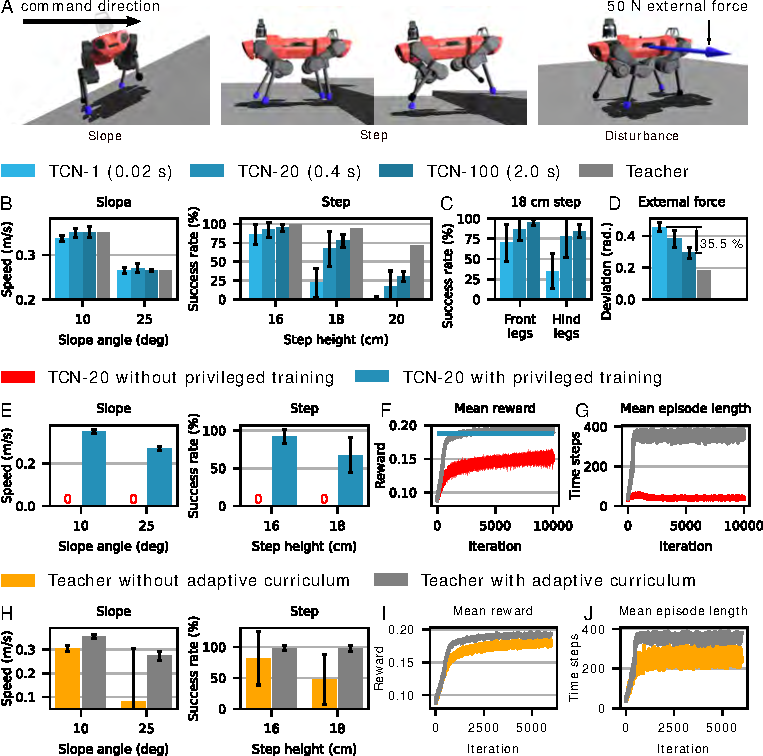
\includegraphics[width=\textwidth]{img/figure5.pdf}
    \caption{\textbf{消融实验（Ablation Studies）。}
    本文使用不同随机种子对每个模型训练5次。误差条表示\unit[95]{\%}置信区间。
    (\textbf{A}) 测试设置。
    机器人被命令在指定方向（黑色箭头）前进\unit[10]{s}。
    每个测试进行100次试验。
    在台阶测试中，如果机器人的前后腿均成功翻越台阶，则试验视为成功。
    机器人以随机关节构型初始化。
    偏航角在斜坡测试中从$U(-\pi,\pi)$采样，在其他测试中从$U(-\pi/6,\pi/6)$采样。
    足部与地面之间的摩擦系数从$U(0.4,1.0)$采样。外部力在横向方向上施加\unit[5]{s}。
    (\textbf{B-D}) TCN-$N$编码器中记忆长度$N$的重要性。
    (\textbf{E-G})~特权训练的重要性。
    (\textbf{F})~教师（灰色）和直接训练（无特权训练）的TCN-20学生（红色）的学习曲线。作为对比，蓝线表示通过特权训练训练的TCN-20学生的平均奖励。奖励通过在均匀采样的地形上运行每个策略来计算。
    (\textbf{H-J})~自适应课程的重要性。
    }\label{fig:5}
\end{figure*}
\begin{figure*}
    \centering
    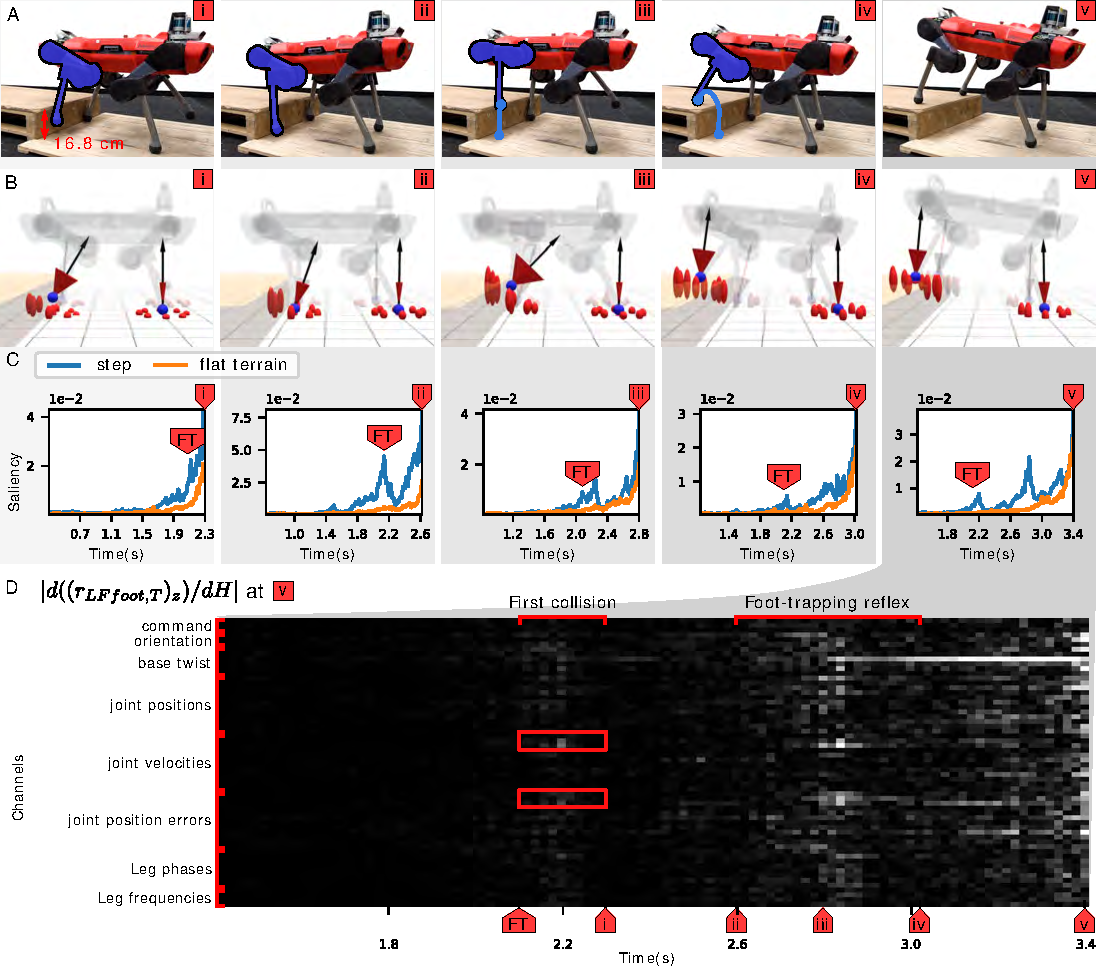
\includegraphics[width=\textwidth]{img/figure6.pdf}
    \caption{\textbf{涌现的足部卡陷反射分析。} FT表示LF足部与台阶的首次接触（足部卡陷事件）。
    (\textbf{A}) LF足部撞击台阶，随后在下一个摆动相中展现出更高的离地高度以翻越台阶（ii-iv）。
    (\textbf{B}) 从TCN嵌入中重建的地形信息。
     红色椭球：估计的足部周围地形形状。椭球中心指估计的地形高程，垂直长度表示不确定性（标准差）。黑色箭头：接触足部处的地形法线。红色锥体：法线估计的不确定性。蓝色球体：估计的接触足部。
    (\textbf{C}) 不同时刻的输入显著性。峰值表明TCN策略关注大约在\unit[2.1]{s}时发生的足部卡陷（FT）。橙色曲线（平坦地形）显示了在相似步态相位下平坦地形上计算的显著性值。
    (\textbf{D}) 在\unit[3.4]{s}时跨输入通道展开的显著性图。红色框表示LF腿在与台阶碰撞时刻的关节测量值。}
    \label{fig:6}
\end{figure*}


\subsection*{方法验证}
本文通过消融实验（Ablation Studies）来证明本文方法每个组成部分的必要性：（1）学生策略使用序列模型，（2）特权训练，以及（3）自适应地形课程。

\subsubsection*{本体感知控制中的记忆}

本文通过TCN架构评估在本体感知控制器中加入记忆的重要性~\cite{bai2018empirical}。
记TCN-$N$为感受野为$N$个时间步的TCN。本文使用的网络架构详见表S5。
本文在专为聚焦特定能力而设计的诊断性设置中测试控制器。具体而言，本文测试了在斜坡上的全向运动、翻越离散台阶以及对外部干扰的鲁棒性（图~\ref{fig:5}A）。

图~\ref{fig:5}B-D总结了记忆长度$N$的重要性。在这些实验中，$N$从1（对应20 ms的记忆）变化到100（2 s的本体感知记忆）。后者是本文部署控制器中使用的默认设置。

如图~\ref{fig:5}B所示，记忆长度在均匀斜坡设置中没有显著影响。记忆长度对控制器翻越台阶的能力有显著影响（图~\ref{fig:5}B-C）。具有更长记忆的控制器能够处理更高的台阶。如图~\ref{fig:5}C所示，有限记忆控制器的失败率在后腿遇到台阶时特别高。
具有更长记忆的控制器还能调整后腿轨迹以确保更高的离地高度。

图~\ref{fig:5}D显示，具有更长记忆的控制器对外部干扰更鲁棒。
本文在直行过程中对基座横向施加\unit[50]{N}的外部力，持续\unit[5]{s}，并评估由此产生的与预期运动方向的偏差。TCN-100控制器的偏差比TCN-1低\unit[35.5]{\%}。

\subsubsection*{特权训练}

现在本文评估特权训练的重要性。作为基线方法，本文直接训练TCN-20策略，不使用两阶段特权训练协议。该策略使用与教师训练相同的奖励和超参数通过TRPO~\cite{schulman2015trust}训练。将此基线方法与通过特权学习训练的相同TCN-20架构进行比较。

结果总结在图~\ref{fig:5}E-G中。图~\ref{fig:5}E显示基线方法未能通过诊断测试：它无法在斜坡上运动或翻越台阶。
图~\ref{fig:5}F显示，在训练过程中，基线方法未能达到与具有特权信息的教师MLP架构或通过特权学习训练的本体感知TCN-20架构（与基线方法相同，无特权信息）相当的奖励。
图~\ref{fig:5}G显示了训练期间的平均回合长度，表明基线方法未能学会平衡和运动。

\subsubsection*{自适应地形课程}
现在本文评估自适应地形课程对教师训练的影响。
训练中使用的地形（具体为丘陵、台阶和楼梯）如图~\ref{fig:4}B所示。
作为基线方法，本文使用从$\mathcal{C}$中均匀采样的随机生成地形（见表S2）训练教师。
如图~\ref{fig:5}H所示，在没有自适应课程的情况下训练时，测试地形上的成功率显著降低。
图~\ref{fig:5}I显示，没有自适应课程训练的教师在较低的奖励水平上达到平台期。在整个训练过程中，没有自适应课程训练的模型的平均回合长度更短（图~\ref{fig:5}J）。
这是因为均匀采样更可能抽取到被训练策略无法成功穿越的地形。在这些地形上，策略过早失败，因此获得的训练信号较少。自适应课程调节采样地形的难度，以最大化每个回合的教学效益。本文在补充材料第S6节中提供了对自适应课程的额外评估。


\subsection*{对涌现行为的进一步分析}\label{supp:foot-trapping}
本文进一步分析本体感知策略如何适应不同情境。

为了研究本体感知策略如何感知环境，本文训练了一个解码器网络，从训练好的TCN策略中间层的输出中重建特权信息$x_t\in X$。$x_t$包含学生策略无法直接观测的信息，如接触状态、地形形状和外部干扰。对于足部接触状态的分类，本文使用标准交叉熵损失函数。对于其他状态的回归，本文预测每个分量的均值$m_i$和标准差$\sigma_i$，并使用负高斯对数似然损失来量化TCN表示中编码的不确定性~\cite{kendall2017uncertainties}：
\begin{equation}
    \mathcal{L} = \sum_{i \in \dim (X \setminus \text{contact states})} \frac{(m_i-m_i^{gt})^2}{2\sigma_i^2} + \log(\sigma_i)
\end{equation} 并添加权重衰减。上标$gt$指仿真中生成的真实值。注意，策略网络的参数在解码器训练期间保持固定。因此，解码器网络不用于策略训练。它仅提供对训练后TCN策略所编码信息的洞察。

在图~\ref{fig:6}中，本文提供了足部卡陷反射运动的快照（图~\ref{fig:6}A）和重建的特权信息。在图~\ref{fig:6}B中，本文展示了重建的地形几何和足部接触状态。当LF足部与台阶碰撞时，前腿前方估计的高程增加，其不确定性增长（i+ii）。估计的高程和法向量在足部卡陷反射期间适应台阶（iii+iv）。成功上台阶后，地形不确定性仍然较高（v），表明对未来粗糙地形的预期。此外，解码器网络能够检测水平面和垂直面上的足部接触，同时成功识别正面碰撞，如估计的地形法向量所示（i+iii）。从本体感知历史编码中重建显式环境信息的能力强烈表明TCN策略学会了构建环境的内部表示并用于决策。本文在补充材料第S7节中提供了更多重建特权信息的示例。

本文随后分析本体感知策略如何利用过去的观测。本文计算输入$H \in \mathbb{R}^{60 \times N}$的显著性图，并可视化策略在翻越台阶时对输入每个元素的敏感性~\cite{simonyan2013deep}。
$H$的每一列是一个本体感知测量值$h \in \mathbb{R}^{60}$，本文堆叠$N$个测量值（历史长度 = $\unit[0.02]{s}\times N$）。
本文定义第$i$个测量值（$i \in [0, N]$）的显著性值为

\begin{equation}
    M_i = \sum_{j \in channels}(\lvert d((r_{f,T})_z)/dH_{i,j} \rvert) \in \mathbb{R},
\end{equation}

其中$(r_{f,T})_z$指足部$f$的高度指令。
本文计算$(r_{f,T})_z$的值是因为本文关注离地高度的变化。
$M_i$可以解释为输出对第$i$个测量值的敏感性。
由于本文使用一维时序卷积，输出在$\mathbb{R}^{N}$中，即$H$的每一行被视为一个通道。

在图~\ref{fig:6}C中，可以看到足部卡陷事件（FT）处的显著性值在上台阶过程中保持较高。
策略可以直接访问足部卡陷时刻的测量值，并在后续摆动相中加以利用。
这在图~\ref{fig:6}D的红色框中突出显示。
策略关注在足部卡陷事件处测量的LF腿关节状态。


\section{致谢}
\textbf{资助}
本项目部分由英特尔智能系统网络、瑞士国家科学基金会（SNF）通过国家机器人研究能力中心、欧洲研究委员会（ERC）在欧盟地平线2020研究与创新计划下（资助协议号852044和780883）资助。本工作作为ANYmal Research（一个推进腿足机器人学的社区）的一部分进行。
\textbf{作者贡献}
J.L制定了训练和控制方法的主要思路，实现了控制器，搭建了仿真环境，并训练了控制策略。
J.L进行了室内实验。
J.H协助搭建仿真环境。
J.L和L.W共同进行了室外实验。
J.L、J.H、L.W、M.H和V.K完善了想法，参与了实验设计并分析了数据。
\textbf{利益冲突} 作者声明无竞争利益。
\textbf{数据和材料可用性} 评估论文结论所需的所有（其他）数据均在论文或补充材料中提供。其他材料可在\href{https://github.com/leggedrobotics/learning_quadrupedal_locomotion_over_challenging_terrain_supplementary}{\url{https://github.com/leggedrobotics/learning_quadrupedal_locomotion_over_challenging_terrain_supplementary}}找到。


\section*{补充材料}
\makebox[1.8cm][l]{第S1节.} 符号说明 \\
\makebox[1.8cm][l]{第S2节.} 实现细节\\
\makebox[1.8cm][l]{第S3节.} 足部轨迹生成器\\
\makebox[1.8cm][l]{第S4节.} 教师策略训练的奖励函数 \\
\makebox[1.8cm][l]{第S5节.} 参数化地形\\
\makebox[1.8cm][l]{第S6节.} 自适应地形课程的定性评估\\
\makebox[1.8cm][l]{第S7节.} 不同情境下特权信息的重建 \\
\makebox[1.8cm][l]{第S8节.} 循环神经网络学生策略 \\
\makebox[1.8cm][l]{第S9节.} 学生训练中潜在表示损失的消融实验\\
\makebox[1.8cm][l]{算法S1.} 带自动地形课程的教师训练\\
\makebox[1.8cm][l]{图S1.} 自适应课程示意图。\\
\makebox[1.8cm][l]{图S2.} 不同情境下重建的特权信息。\\
\makebox[1.8cm][l]{图S3.} 本体感知控制器的神经网络架构比较 \\
\makebox[1.8cm][l]{表S1.} 训练计算时间 \\
\makebox[1.8cm][l]{表S2.} 仿真地形的参数空间$\mathcal{C}$\\
\makebox[1.8cm][l]{表S3.} 自动地形课程的超参数\\
\makebox[1.8cm][l]{表S4.} 本体感知控制器和特权信息的状态表示 \\
\makebox[1.8cm][l]{表S5.} 神经网络架构 \\
\makebox[1.8cm][l]{表S6.} 学生策略的网络参数设置及训练时间\\
\makebox[1.8cm][l]{表S7.} 教师策略训练的超参数 \\
\makebox[1.8cm][l]{表S8.} 学生策略训练的超参数 \\
\makebox[1.8cm][l]{表S9.} 解码器训练的超参数\\
\href{https://youtu.be/txjqn8h6pjU}{\makebox[1.8cm][l]{Movie S1.} 森林中的部署} \\
\href{https://youtu.be/Xnn4sVSpSh0}{\makebox[1.8cm][l]{Movie S2.} 在不稳定碎片上的运动} \\
\href{https://youtu.be/tPixnjLbTvE}{\makebox[1.8cm][l]{Movie S3.} 台阶实验}   \\
\href{https://youtu.be/3Nr47MXCFO0}{\makebox[1.8cm][l]{Movie S4.} 负载实验}  \\
\href{https://youtu.be/aMPwB3t4idU}{\makebox[1.8cm][l]{Movie S5.} 足部打滑实验}

\begin{thebibliography}{10}

\bibitem{jenelten2019dynamic}
F.~Jenelten, J.~Hwangbo, F.~Tresoldi, C.~D. Bellicoso, M.~Hutter, Dynamic
  locomotion on slippery ground, {\it IEEE Robotics and Automation Letters\/}
  4170--4176 (2019).

\bibitem{bledt2018contact}
G.~Bledt, P.~M. Wensing, S.~Ingersoll, S.~Kim, Contact model fusion for
  event-based locomotion in unstructured terrains, {\it 2018 IEEE International
  Conference on Robotics and Automation (ICRA)\/} (IEEE, 2018).

\bibitem{focchi2020heuristic}
M.~Focchi, R.~Orsolino, M.~Camurri, V.~Barasuol, C.~Mastalli, D.~G. Caldwell,
  C.~Semini.
\newblock Heuristic planning for rough terrain locomotion in presence of
  external disturbances and variable perception quality.
\newblock {\it Advances in Robotics Research: From Lab to Market\/} (Springer,
  2020),  165--209.

\bibitem{Reher2019}
J.~Reher, W.~Ma, A.~D. Ames, Dynamic walking with compliance on a {Cassie}
  bipedal robot, {\it European Control Conference\/},  2589--2595 ({IEEE},
  2019).

\bibitem{gong2019feedback}
Y.~Gong, R.~Hartley, X.~Da, A.~Hereid, O.~Harib, J.~Huang, J.~W. Grizzle,
  Feedback control of a {Cassie} bipedal robot: Walking, standing, and riding a
  {Segway}, {\it American Control Conference\/},  4559--4566 (IEEE, 2019).

\bibitem{hwangbo2016probabilistic}
J.~Hwangbo, C.~D. Bellicoso, P.~Fankhauser, M.~Huttery, Probabilistic foot
  contact estimation by fusing information from dynamics and
  differential/forward kinematics, {\it 2016 IEEE/RSJ International Conference
  on Intelligent Robots and Systems (IROS)\/},  3872--3878 (IEEE, 2016).

\bibitem{camurri2017probabilistic}
M.~Camurri, M.~Fallon, S.~Bazeille, A.~Radulescu, V.~Barasuol, D.~G. Caldwell,
  C.~Semini, Probabilistic contact estimation and impact detection for state
  estimation of quadruped robots, {\it IEEE Robotics and Automation Letters\/}
  1023--1030 (2017).

\bibitem{focchi2018slip}
M.~Focchi, V.~Barasuol, M.~Frigerio, D.~G. Caldwell, C.~Semini.
\newblock Slip detection and recovery for quadruped robots.
\newblock {\it Robotics Research\/} (Springer, 2018),  185--199.

\bibitem{Bloesch2013}
M.~Bl{\"{o}}sch, C.~Gehring, P.~Fankhauser, M.~Hutter, M.~A. Hoepflinger,
  R.~Siegwart, State estimation for legged robots on unstable and slippery
  terrain, {\it 2013 {IEEE/RSJ} International Conference on Intelligent Robots
  and Systems\/},  6058--6064 ({IEEE}, 2013).

\bibitem{gehring2015dynamic}
C.~Gehring, C.~D. Bellicoso, S.~Coros, M.~Bloesch, P.~Fankhauser, M.~Hutter,
  R.~Siegwart, Dynamic trotting on slopes for quadrupedal robots, {\it 2015
  IEEE/RSJ International Conference on Intelligent Robots and Systems
  (IROS)\/},  5129--5135 (IEEE, 2015).

\bibitem{hartley2018legged}
R.~Hartley, J.~Mangelson, L.~Gan, M.~G. Jadidi, J.~M. Walls, R.~M. Eustice,
  J.~W. Grizzle, Legged robot state-estimation through combined forward
  kinematic and preintegrated contact factors, {\it 2018 IEEE International
  Conference on Robotics and Automation (ICRA)\/},  1--8 (IEEE, 2018).

\bibitem{hwangbo2019learning}
J.~Hwangbo, J.~Lee, A.~Dosovitskiy, D.~Bellicoso, V.~Tsounis, V.~Koltun,
  M.~Hutter, Learning agile and dynamic motor skills for legged robots, {\it
  Science Robotics\/} p. eaau5872 (2019).

\bibitem{haarnoja2018learning}
T.~Haarnoja, S.~Ha, A.~Zhou, J.~Tan, G.~Tucker, S.~Levine, Learning to walk via
  deep reinforcement learning, {\it Robotics: Science and Systems\/} (2019).

\bibitem{xie2019iterative}
Z.~Xie, P.~Clary, J.~Dao, P.~Morais, J.~Hurst, M.~van~de Panne, Learning
  locomotion skills for {Cassie}: Iterative design and sim-to-real, {\it
  Conference on Robot Learning\/} (2019).

\bibitem{lee2019robust}
J.~Lee, J.~Hwangbo, M.~Hutter, Robust recovery controller for a quadrupedal
  robot using deep reinforcement learning, {\it arXiv:1901.07517\/}  (2019).

\bibitem{tan2018sim}
J.~Tan, T.~Zhang, E.~Coumans, A.~Iscen, Y.~Bai, D.~Hafner, S.~Bohez,
  V.~Vanhoucke, Sim-to-real: Learning agile locomotion for quadruped robots,
  {\it Robotics: Science and Systems\/} (2018).

\bibitem{yang2019data}
Y.~Yang, K.~Caluwaerts, A.~Iscen, T.~Zhang, J.~Tan, V.~Sindhwani, Data
  efficient reinforcement learning for legged robots, {\it Conference on Robot
  Learning\/} (2019).

\bibitem{ha2020learning}
S.~Ha, P.~Xu, Z.~Tan, S.~Levine, J.~Tan, Learning to walk in the real world
  with minimal human effort, {\it arXiv:2002.08550\/}  (2020).

\bibitem{Peng2020}
X.~B. Peng, E.~Coumans, T.~Zhang, T.-W. Lee, J.~Tan, S.~Levine, Learning agile
  robotic locomotion skills by imitating animals, {\it arXiv:2004.00784\/}
  (2020).

\bibitem{hutter2016anymal}
M.~Hutter, C.~Gehring, D.~Jud, A.~Lauber, C.~D. Bellicoso, V.~Tsounis,
  J.~Hwangbo, K.~Bodie, P.~Fankhauser, M.~Bloesch, R.~Diethelm, S.~Bachmann,
  A.~Melzer, M.~A. H{\"{o}}pflinger, {ANYmal} - a highly mobile and dynamic
  quadrupedal robot, {\it {IEEE/RSJ} International Conference on Intelligent
  Robots and Systems\/},  38--44 ({IEEE}, 2016).

\bibitem{peng2018sim}
X.~B. Peng, M.~Andrychowicz, W.~Zaremba, P.~Abbeel, Sim-to-real transfer of
  robotic control with dynamics randomization, {\it IEEE International
  Conference on Robotics and Automation (ICRA)\/} (IEEE, 2018).

\bibitem{bai2018empirical}
S.~Bai, J.~Z. Kolter, V.~Koltun, An empirical evaluation of generic
  convolutional and recurrent networks for sequence modeling, {\it
  arXiv:1803.01271\/}  (2018).

\bibitem{chenlearning}
D.~Chen, B.~Zhou, V.~Koltun, P.~Kr\"ahenb\"uhl, Learning by cheating, {\it
  Conference on Robot Learning\/} (2019).

\bibitem{brant2017minimal}
J.~C. Brant, K.~O. Stanley, Minimal criterion coevolution: a new approach to
  open-ended search, {\it Genetic and Evolutionary Computation Conference\/},
  67--74 (2017).

\bibitem{wang2019paired}
R.~Wang, J.~Lehman, J.~Clune, K.~O. Stanley, Paired open-ended trailblazer
  (poet): Endlessly generating increasingly complex and diverse learning
  environments and their solutions, {\it arXiv:1901.01753\/}  (2019).

\bibitem{bellicoso2018dynamic}
C.~D. Bellicoso, F.~Jenelten, C.~Gehring, M.~Hutter, Dynamic locomotion through
  online nonlinear motion optimization for quadrupedal robots, {\it IEEE
  Robotics and Automation Letters\/}  2261--2268 (2018).

\bibitem{fankhauser2014robot}
P.~Fankhauser, M.~Bloesch, C.~Gehring, M.~Hutter, R.~Siegwart.
\newblock Robot-centric elevation mapping with uncertainty estimates.
\newblock {\it Mobile Service Robotics\/} (World Scientific, 2014),  433--440.

\bibitem{collins2005efficient}
S.~Collins, A.~Ruina, R.~Tedrake, M.~Wisse, Efficient bipedal robots based on
  passive-dynamic walkers, {\it Science\/}  1082--1085 (2005).

\bibitem{vision60blind}
{Ghost Robotics}, Vision 60: Latest blind-mode stress testing of {V60} legged
  robot, \url{www.youtube.com/watch?v=tQsLauQWp8M} (2019).

\bibitem{hwangbo2018per}
J.~Hwangbo, J.~Lee, M.~Hutter, Per-contact iteration method for solving contact
  dynamics, {\it IEEE Robotics and Automation Letters\/}  895--902 (2018).

\bibitem{coumans2013bullet}
E.~Coumans, others, Bullet physics library, Open source:
  \url{bulletphysics.org} (2013).

\bibitem{smith2005open}
R.~Smith, others, Open dynamics engine, Open source: \url{ode.org} (2005).

\bibitem{Alexander2003}
R.~M. Alexander, {\it Principles of Animal Locomotion\/} (Princeton University
  Press, 2003).

\bibitem{iscen2018policies}
A.~Iscen, K.~Caluwaerts, J.~Tan, T.~Zhang, E.~Coumans, V.~Sindhwani,
  V.~Vanhoucke, Policies modulating trajectory generators, {\it Conference on
  Robot Learning\/},  916--926 (2018).

\bibitem{barasuol2013reactive}
V.~Barasuol, J.~Buchli, C.~Semini, M.~Frigerio, E.~R. De~Pieri, D.~G. Caldwell,
  A reactive controller framework for quadrupedal locomotion on challenging
  terrain, {\it 2013 IEEE International Conference on Robotics and
  Automation\/},  2554--2561 (IEEE, 2013).

\bibitem{schulman2015trust}
J.~Schulman, S.~Levine, P.~Abbeel, M.~Jordan, P.~Moritz, Trust region policy
  optimization, {\it International Conference on Machine Learning\/},
  1889--1897 (2015).

\bibitem{bloesch2013state}
M.~Bloesch, M.~Hutter, M.~A. Hoepflinger, S.~Leutenegger, C.~Gehring, C.~D.
  Remy, R.~Siegwart, State estimation for legged robots-consistent fusion of
  leg kinematics and imu, {\it Robotics\/}  17--24 (2013).

\bibitem{ross2011reduction}
S.~Ross, G.~Gordon, D.~Bagnell, A reduction of imitation learning and
  structured prediction to no-regret online learning, {\it International
  Conference on Artificial Intelligence and Statistics\/},  627--635 (2011).

\bibitem{florensa2018automatic}
C.~Florensa, D.~Held, X.~Geng, P.~Abbeel, Automatic goal generation for
  reinforcement learning agents, {\it International Conference on Machine
  Learning\/},  1514--1523 (2018).

\bibitem{lehman2010revising}
J.~Lehman, K.~O. Stanley, Revising the evolutionary computation abstraction:
  minimal criteria novelty search, {\it Genetic and Evolutionary Computation
  Conference\/},  103--110 (2010).

\bibitem{matiisen2019teacher}
T.~Matiisen, A.~Oliver, T.~Cohen, J.~Schulman, Teacher-student curriculum
  learning, {\it IEEE transactions on neural networks and learning systems\/}
  (2019).

\bibitem{yu2018learning}
W.~Yu, G.~Turk, C.~K. Liu, Learning symmetric and low-energy locomotion, {\it
  ACM Transactions on Graphics (TOG)\/} p. 144 (2018).

\bibitem{akkaya2019solving}
I.~Akkaya, M.~Andrychowicz, M.~Chociej, M.~Litwin, B.~McGrew, A.~Petron,
  A.~Paino, M.~Plappert, G.~Powell, R.~Ribas, others, Solving rubik's cube with
  a robot hand, {\it arXiv:1910.07113\/}  (2019).

\bibitem{chavez2018learning}
R.~O. Chavez-Garcia, J.~Guzzi, L.~M. Gambardella, A.~Giusti, Learning ground
  traversability from simulations, {\it IEEE Robotics and Automation Letters\/}
   1695--1702 (2018).

\bibitem{kendall2017uncertainties}
A.~Kendall, Y.~Gal, What uncertainties do we need in bayesian deep learning for
  computer vision?, {\it Advances in neural information processing systems\/},
  5574--5584 (2017).

\bibitem{simonyan2013deep}
K.~Simonyan, A.~Vedaldi, A.~Zisserman, Deep inside convolutional networks:
  Visualising image classification models and saliency maps, {\it
  arXiv:1312.6034\/}  (2013).

\bibitem{pratt1995series}
G.~A. Pratt, M.~M. Williamson, Series elastic actuators, {\it IEEE/RSJ
  International Conference on Intelligent Robots and Systems\/},  399--406
  (1995).

\bibitem{smelik2009survey}
R.~M. Smelik, K.~J. De~Kraker, T.~Tutenel, R.~Bidarra, S.~A. Groenewegen, A
  survey of procedural methods for terrain modelling, {\it Proceedings of the
  CASA Workshop on 3D Advanced Media In Gaming And Simulation (3AMIGAS)\/},
  25--34 (2009).

\bibitem{lagae2010survey}
A.~Lagae, S.~Lefebvre, R.~Cook, T.~DeRose, G.~Drettakis, D.~S. Ebert, J.~P.
  Lewis, M.~Perlin, M.~Zwicker, A survey of procedural noise functions, {\it
  Computer Graphics Forum\/},  2579--2600 (Wiley Online Library, 2010).

\bibitem{chung2014empirical}
J.~Chung, C.~Gulcehre, K.~Cho, Y.~Bengio, Empirical evaluation of gated
  recurrent neural networks on sequence modeling, {\it arXiv:1412.3555\/}
  (2014).

\bibitem{williams1990efficient}
R.~J. Williams, J.~Peng, An efficient gradient-based algorithm for on-line
  training of recurrent network trajectories, {\it Neural Computation\/}
  490--501 (1990).

\bibitem{kingma2014adam}
D.~P. Kingma, J.~Ba, Adam: A method for stochastic optimization, {\it
  International Conference on Learning Representations\/} (2015).

\end{thebibliography}


\clearpage
\newpage

\setcounter{table}{0}
\makeatletter
\renewcommand{\thetable}{S\@arabic\c@table}
\makeatother

\setcounter{figure}{0}
\makeatletter
\renewcommand{\thefigure}{S\@arabic\c@figure}
\makeatother

\setcounter{algorithm}{0}
\makeatletter
\renewcommand{\thealgorithm}{S\@arabic\c@algorithm}
\makeatother



\section*{补充材料}
\subsection*{S1. 符号说明}
\makebox[1.2cm]{$\hat{(\cdot)}$} 归一化向量\\
\makebox[1.2cm]{$\dot{(\cdot)}$} 一阶导数\\
\makebox[1.2cm]{$\bar{(\cdot)}$} 教师的量\\
\makebox[1.2cm]{${(\cdot)}_T$} 目标量\\
\makebox[1.2cm]{$^C_{AB}v$} $B$坐标系相对于$A$坐标系的线速度\\
\makebox[1.2cm]{}\. 在$C$坐标系中表示\\
\makebox[1.2cm]{$c_T$} 地形参数向量\\
\makebox[1.2cm]{$\omega$} 角速度\\
\makebox[1.2cm]{$\tau$} 关节力矩\\
\makebox[1.2cm]{$\theta$} 关节角度\\
\makebox[1.2cm]{$\psi$} 偏航角\\
\makebox[1.2cm]{$\phi$} 腿部相位\\
\makebox[1.2cm]{$f$} 腿部频率\\
\makebox[1.2cm]{$r_f$} 足部的线位置\\
\makebox[1.2cm]{$e_g$} 重力向量\\
\makebox[1.2cm]{$H$} 水平坐标系\\
\makebox[1.2cm]{$g_i$} 第$i$个可能接触对的间隙函数\\
\makebox[1.2cm]{$I_{c}$} 所有接触的索引集合\\
\makebox[1.2cm]{$I_{c,body}$} 身体接触的索引集合\\
\makebox[1.2cm]{$I_{c,foot}$} 足部接触的索引集合\\
\makebox[1.2cm]{$I_{swing}$} 摆动腿的索引集合\\
\makebox[1.2cm]{$\lvert \cdot \rvert$} 集合的基数或$l_1$范数\\
\makebox[1.2cm]{$\lvert\lvert \cdot \rvert\rvert$} $l_2$范数\\

\subsection*{S2. 实现细节}\label{impl_details}
RaiSim仿真器~\cite{hwangbo2018per}用于刚体和接触动力学仿真。
为每台机器人训练执行器网络~\cite{hwangbo2019learning}，以模拟关节处的串联弹性执行器（Series Elastic Actuator, SEA）~\cite{pratt1995series}。
执行器模型的输入是一个6维实值向量，包含当前时间步$t$以及两个过去状态（$t - \unit[0.01]{s}$和$t - \unit[0.02]{s}$）的关节位置误差和速度。
特征选择按文献~\cite{hwangbo2019learning}完成。
%and proven to be sufficient to learn the dynamics of SEAs in the operating range of our tasks.

由于多项研究表明动态属性的随机化可提高策略的鲁棒性~\cite{hwangbo2019learning,tan2018sim}，本文也对若干物理量进行了随机化，教师策略在训练过程中可以访问这些值。
本文在训练过程中施加了干扰，对足部与地形之间的摩擦系数进行了随机化，并对观测添加了加性噪声。
% we did not apply dynamic randomization as we did not observe any difference.

教师策略的训练过程如算法S1所示。超参数见表S3。在地形课程的实现中，本文每$N_{evaluate}$次策略迭代更新一次课程以减少方差。本文假设在$N_{evaluate}$次迭代内，策略的性能相似。使用较慢的更新率时，公式6的测量概率变为
\begin{equation}
    \Pr(y_j^k|c_{T,j}^k)
    \approx
    \sum_{}^{N_{evaluate}}
     \sum_{}^{N_{traj}}
     \frac{\mathbbm{1} (Tr(c_{T,j}^k,\pi) \in [0.5, 0.9])}{ N_{traj} N_{evaluate}}.
\label{measurement_model3}\end{equation} 此外，本文利用回放记忆（Replay Memory）来防止粒子滤波退化并避免灾难性遗忘。

控制器通过状态机在"静止站立"状态和运动状态之间切换。当零指令持续\unit[0.5]{s}时，本文将基频$f_0$设为零，从而停止FTG，机器人在地形上静止站立。
当接收到方向指令或基座线速度超过\unit[0.3]{m/s}（用于干扰抑制）时，$f_0$设为\unit[1.25]{Hz}。状态机包含在训练环境中。

部署期间，基座速度和方向由依赖惯性测量和腿部运动学的状态估计器估计~\cite{bloesch2013state}。

神经网络策略在机器人集成的机载CPU（Intel i7-5600U, 2.6 -- 3.2GHz, 双核64位）上以400 Hz运行。使用Tensorflow C++ API进行机载推理。


\begin{algorithm}
\caption{带自动地形课程的教师训练}
\begin{algorithmic}[1]
\State 初始化回放记忆，从$\mathcal{C}$中均匀采样$N_{particle}$个$c_{T,0}$（表S2），$i,j  = 0$.
\Repeat
\For{$0 \leq k \leq N_{evaluate}$}
\For{$0 \leq l \leq N_{particle}$}
\For{$0 \leq m \leq N_{traj}$}
% \Comment{This loop runs in parallel}
\State 使用$c_{T,j}^l$生成地形
\State 在随机位置初始化机器人
\State 运行策略$\pi_{i}$
\State 计算每个状态转移的
\par \hskip\algorithmicindent \hskip\algorithmicindent \hskip\algorithmicindent 可穿越性标签（公式~2）
\State 保存分数和轨迹
\EndFor
\EndFor
\State 使用TRPO更新策略~\cite{schulman2015trust}
\State $i = i + 1$
\EndFor

\For{$0 \leq l \leq N_{particle}$}
\State 计算每个参数$c_{T,j}^l$的测量概率
\par \hskip\algorithmicindent （公式~9）
\EndFor
\For{$0 \leq l \leq N_{particle}$}
\State 更新权重$w_{j} = \frac{P(y_i^l|c_{T,j}^l)}{\sum_{m} P(y_i^m|c_{T,j}^m)}$
\EndFor
\State 重采样$N_{particle}$个参数
\State 将$c_{T,j}$追加到回放记忆
\For{$0 \leq l \leq N_{particle}$}
\State 以$p_{replay}$概率从回放记忆中采样
\State 以$p_{transition}$概率将$c^l_{T,j}$移动到$\mathcal{C}$中的相邻值

\EndFor
\State $j = j + 1$
% \State $c_{T,j} = c_{T,j-1} + \epsilon$ for all particles
\Until{收敛}
\end{algorithmic}
\label{algo:TPF}
\end{algorithm}

\subsection*{S3. 足部轨迹生成器}

足部轨迹定义为
\begin{equation}
F(\phi_i) =
\begin{cases}
(h (-2k^3+3k^2) - 0.5) ^{H_i}z  &  k \in [0, 1] \\
(h (2k^3-9k^2+12k-4) - 0.5)  ^{H_i}z &  k \in [1, 2] \\
- 0.5 ^{H_i}z & \text{otherwise},
\end{cases}{}
% \quad \text{where} \quad k = 2\phi / \pi, \, \phi_i = f_i t\pmod{2 \pi} - \pi
\end{equation}
其中$k = 2 (\phi_i - \pi) / \pi$，$h$是最大足部高度的参数。
摆动相（$k \in [0, 2)$）期间的每个分段是连接最高点和最低点的三次厄米样条，在连接点处一阶导数为零。
其他周期函数如$ h_i \sin(\phi_i)$也可用于FTG。
通过一组合理调整的$f_0$、$h$和$\phi_{i,0}$，四足机器人可以在原地稳定踏步。
在本文的设置中，$f_0$ = 1.25，$h$ = \unit[0.2]{m}，$\phi_{i,0}$从$U(0, 2\pi)$采样。


\subsection*{S4. 教师策略训练的奖励函数}

奖励函数定义为
$0.05r_{lv} + 0.05r_{av} + 0.04r_b + 0.01r_{fc} + 0.02r_{bc} + 0.025 r_s+ 2 \cdot 10^{-5} r_{\tau}.$
% $2.5r_{lv} + 2.5r_{av} + 2.0r_b + 0.5r_{fc}+1.0r_{bc}+1.2r_s+0.001r_{tau}.$
各项定义如下。

\begin{itemize}
    \item 线速度奖励（$r_{lv}$）：该项最大化$v_{pr} = (^B_{IB}v)_{xy} \cdot (^{B}_{IB} \hat{v}_{T})_{xy}$，即基座线速度在指令方向上的投影。
    \begin{equation}
    r_{lv} \coloneqq
        \begin{cases}
            \exp{(-2.0 (v_{pr} - 0.6)^2)} & v_{pr} < 0.6 \\
            1.0  & v_{pr} \geq 0.6 \\
           % 0.0  & \lvert \lvert  (^B_{IB}\hat{v})_{xy} \rvert \rvert = 0.0 \\
            0.0  & \text{zero command}\\
        \end{cases}.
    \end{equation}
    速度阈值定义为\unit[0.6]{m/s}，这是现有控制器~\cite{bellicoso2018dynamic}在平坦地面上可达到的最大速度。

   \item 角速度奖励（$r_{av}$）：本文鼓励智能体在$(^{B}_{IB}\hat{\omega}_{T})_{z}$非零时尽可能快地沿基座$z$轴转向。定义为
    \begin{equation}
    r_{av} \coloneqq
        \begin{cases}
            \exp{(- 1.5 ( \omega_{pr} - 0.6)^2)} & \omega_{pr} < 0.6 \\
            1.0  & \omega_{pr} \geq 0.6 \\
        \end{cases},
    \end{equation}
     其中$\omega_{pr} = (^B_{IB} \omega)_{z} \cdot (^{B}_{IB}\hat{\omega}_{T})_{z}$。

    \item 基座运动奖励（$r_{b}$）：
    该项惩罚垂直于目标方向的速度以及横滚和俯仰角速率，使基座在运动过程中保持稳定。
    \begin{equation}
      r_{b} \coloneqq \exp(- 1.5 v_{o}^2) + \exp( - 1.5 \lvert\lvert(^B_{IB} \omega)_{xy} \rvert\rvert^2)
    \end{equation}
   其中$v_{o} = \lvert\lvert (^B_{IB} v)_{xy} - v_{pr}\cdot (^{B}_{IB} \hat{v}_{T})_{xy} \rvert\rvert$。
    当给定停止指令时，$v_{o}$替换为$\lvert\lvert ^B_{IB} v\rvert\rvert$。

    \item 离地高度奖励（$r_{fc}$）：
    当腿部处于摆动相（即$\phi_i \in [\pi, 2\pi)$）时，机器人应将相应足部抬高到高于周围环境以避免碰撞。
    本文首先定义无碰撞足部的集合为$\mathcal{F}_{clear} = \{ i : r_{f,i} > max(H_{scan, i}) , i \in I_{swing} \}$，
    其中$H_{scan,i}$是第$i$个足部周围的扫描高度集合。
    于是离地成本定义为
    \begin{equation}
        r_{fc} \coloneqq \sum_{i \in I_{swing}}
        (\mathbbm{1}_{\mathcal{F}_{clear}}(i) / \lvert I_{swing} \rvert )
        \in [0.0, 1.0].
    \end{equation}

    \item 身体碰撞奖励（$r_{bc}$）：本文希望惩罚机器人身体部位与地形之间不必要的接触，以避免硬件损坏。
    \begin{equation}
        r_{bc} \coloneqq -\lvert I_{c, body} \backslash I_{c, foot} \rvert.
    \end{equation}

    \item 目标平滑度奖励（$r_{s}$）：
    惩罚目标足部位置的二阶有限差分量，使生成的足部轨迹更平滑。
     \begin{equation}
        r_{s} \coloneqq - \lvert\lvert
        (r_{f,d})_{t} - 2(r_{f,d})_{t-1} + (r_{f,d})_{t-2}
        \rvert\rvert .
    \end{equation}

    \item 力矩奖励（$r_{\tau}$）：本文惩罚关节力矩，以防止部署过程中损坏关节执行器并降低能耗（$\tau \propto \text{electric current}$）。
    \begin{equation}
          r_{\tau} \coloneqq - \textstyle \sum_{i\in joints} \lvert \tau_i \rvert.
    \end{equation}


\end{itemize}


\subsection*{S5. 参数化地形}
生成能够呈现代表性挑战（如足部打滑和足部卡陷）的训练环境至关重要。
为了高效合成随机地形，本文使用程序化生成技术~\cite{smelik2009survey}。
该方法通过改变一组地形参数$c_T \in \mathcal{C}$来生成大量不同的地形。
下面描述本文工作中使用的三种地形生成器。
地形可视化见图4B，参数空间$\mathcal{C}$的定义见表S2。

\begin{itemize}
  \item \textit{丘陵}地形基于Perlin噪声~\cite{lagae2010survey}。
  地形由三个参数生成：粗糙度、Perlin噪声频率和Perlin噪声振幅。
%   $c_{T} \coloneqq \langle \text{roughness, frequency, amplitude} \rangle$
  输出高度图$hm$的每个元素的高度定义为$hm[i,j] \coloneqq Perlin (c_{T,2}, c_{T,3})[i,j] + U(-c_{T,1}, c_{T,1})$。
  策略在训练过程中在此地形上经历平滑坡道和足部打滑。

  \item \textit{台阶}地形由随机高度的方形台阶组成。每$c_{T,1} \times c_{T,1}$的块内，高度从$U(0, c_{T,2})$采样。
  策略在此地形上经历离散高程变化和足部卡陷。
  \item \textit{楼梯}地形是具有固定宽度和高度的阶梯。机器人初始化在楼梯中间的平坦段（见图~\ref{fig:4}B）。
\end{itemize}
各范围的设定考虑了机器人的运动学约束，例如台阶高度应小于腿长。
在训练过程中，每个回合以不同的随机种子重新生成地形。

\subsection*{S6. 自适应地形课程的定性评估}
自适应课程的行为如图S1所示。
图S1A-C聚焦于\textit{丘陵}地形类型。该地形有三个参数：粗糙度、频率和振幅。
可穿越性（公式3）与期望度（公式4）之间的关系如图S1A-B所示。
不期望的地形要么太简单要么太困难，如图S1A最左和最右图所示。
图S1B-C显示粒子滤波拟合了期望地形的潜在分布，该分布在频率-振幅边际上呈现弓形（中间）。
图S1D聚焦于\textit{楼梯}地形类型，展示了训练过程中地形参数的演化。
粒子滤波拒绝了代表短而陡台阶的参数（左上区域）。课程初始阶段专注于宽而浅的台阶（中间面板，特别是第50-60次迭代），然后扩展到包含更窄台阶的分布（最右面板）。

\subsection*{S7. 不同情境下特权信息的重建}
在图S2中，本文展示了不同情境下解码的特权信息。图S2A显示了穿越潮湿光滑白板时足部与地形之间的估计摩擦系数，如\href{https://youtu.be/aMPwB3t4idU}{Movie~S5}所示。一旦第一只脚开始打滑，估计值立即下降（i），在整个穿越过程中保持较低（ii），并在机器人返回正常地面约\unit[2]{s}后增加（iii）。外部干扰和地形信息也可以从TCN嵌入中重建。
如图S2B所示，当施加未知的\unit[10]{kg}负载时，解码器检测到向下的外部力。
在图S2C所示的穿越茂密植被时，检测到与运动方向相反的力，促使策略抵消并穿过植被。
在图S2C和图S2D所示的自然地形中，高程估计的不确定性显著较高，表明TCN策略编码了地形的粗糙度。


\subsection*{S8. 循环神经网络学生策略}

本文使用TCN架构作为本体感知策略~\cite{bai2018empirical}。作为对比，本文还评估了具有门控循环单元（Gated Recurrent Unit, GRU）的循环网络~\cite{chung2014empirical}。架构详见表S5和S6。
训练GRU学生策略的损失函数定义为
\begin{equation}
\mathcal{L} \coloneqq (\bar{a_t}(o_t, x_t) - a_t(o_t))^2 +  (\bar{l_t}(o_t, x_t) - l_t(o_t))^2.
\end{equation}
为了提高训练的性能和计算效率，本文实现了截断时间反向传播（Truncated Backpropagation Through Time, Truncated BPTT）~\cite{williams1990efficient}。

在如图5A所示的诊断性设置上的性能如图S3所示。
总体而言，基于GRU的控制器的性能介于TCN-20和TCN-100之间。
在斜坡设置中性能与TCN-100相当，但基于GRU的控制器在台阶实验中未能达到TCN-100的性能。

TCN的主要优势在于训练效率。与GRU相比，TCN的训练时间快得多。计算时间见表~\ref{tab:times}。

\subsection*{S9. 学生训练中潜在表示损失的消融实验}

本文检验了公式1中学生策略训练损失函数第二项（潜在向量$l_t$的平方误差损失）的效果。
作为基线方法，本文使用以下损失函数训练学生策略：
\begin{equation}
\mathcal{L} \coloneqq (\bar{a_t}(o_t, x_t) - a_t(o_t, H))^2,
\label{eq:student2}\end{equation}
该函数仅模仿教师策略的输出。

结果如图S3中`TCN-100 naive IL`所示。
在均匀斜坡设置和外部干扰下性能相当。另一方面，消融版本在台阶上的成功率较低。


\begin{figure*}
    \centering
    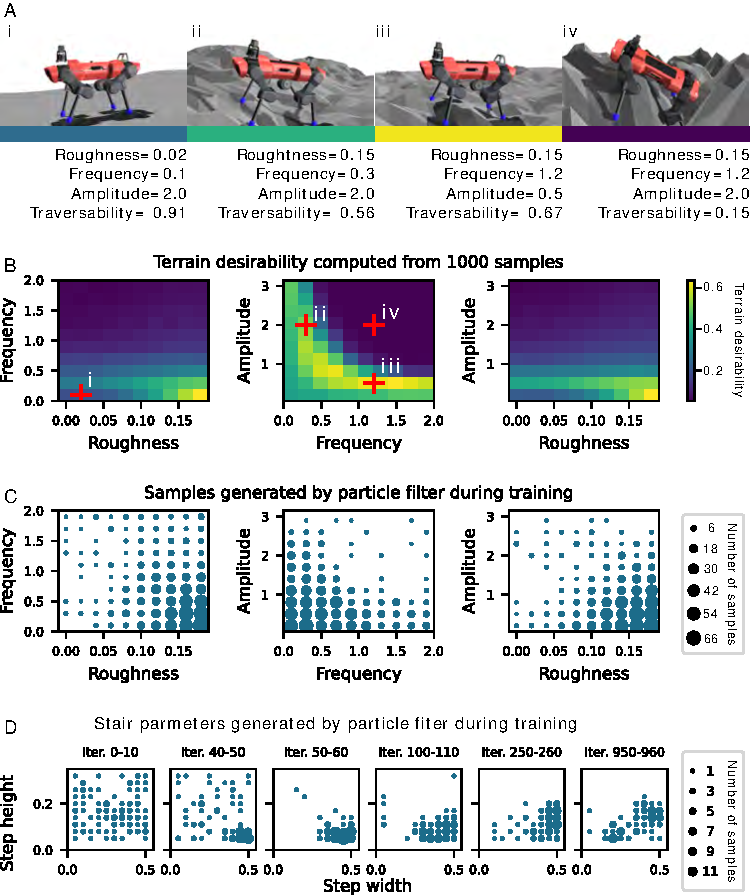
\includegraphics[width=5.0in]{img/figureS1.pdf}
    \caption{\textbf{自适应课程示意图。}
    (\textbf{A}) \textit{丘陵}地形示例。色条表示期望度；深蓝色表示低期望度。
    (\textbf{B}) 根据完全训练好的教师策略生成的1000条轨迹估计的地形期望度。红色叉号对应A中展示的示例。
    (\textbf{C}) 在教师训练的最后100次迭代中由粒子滤波采样的地形分布。
    (\textbf{D}) 训练过程中\textit{楼梯}地形参数的演化。}\label{fig:tpf}
\end{figure*}

\begin{figure*}
    \centering
    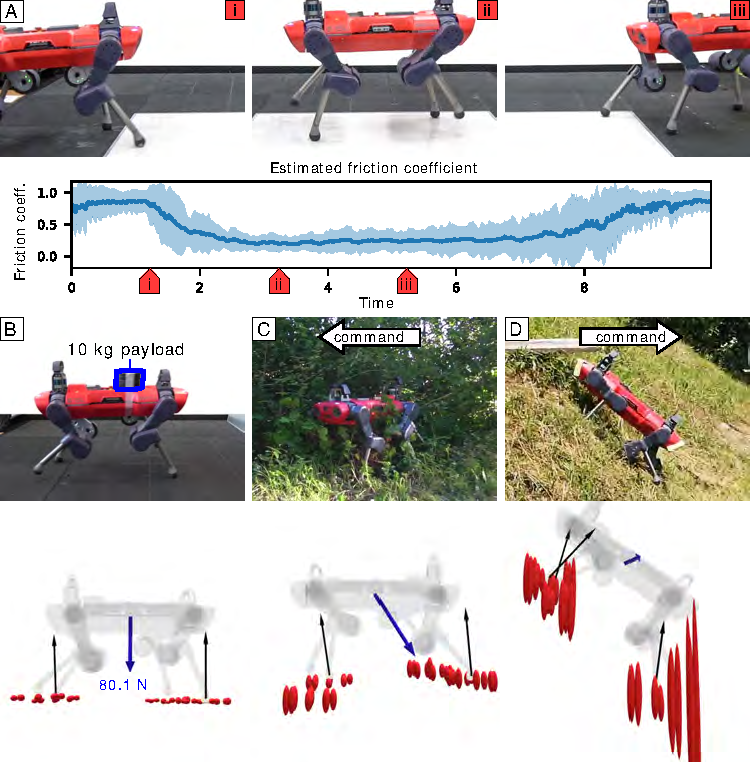
\includegraphics[width=5.0 in]{img/figureS2.pdf}
    \caption{\textbf{不同情境下重建的特权信息。}
    (\textbf{A}) 穿越潮湿白板时足部与地形之间的估计摩擦系数。阴影区域表示\unit[95]{\%}置信区间。(\textbf{B-D}) 不同场景下外部干扰和地形信息的重建。蓝色箭头：估计施加在躯干上的外部力。红色椭球：估计的足部周围地形形状。椭球中心指估计的地形高程，垂直长度表示不确定性（1个标准差）。对于每个足部，8个椭球沿半径为\unit[10]{cm}的圆对称放置。黑色箭头：接触足部处的地形法线。
    }\label{fig:decoding}
\end{figure*}

\begin{figure*}
    \centering
    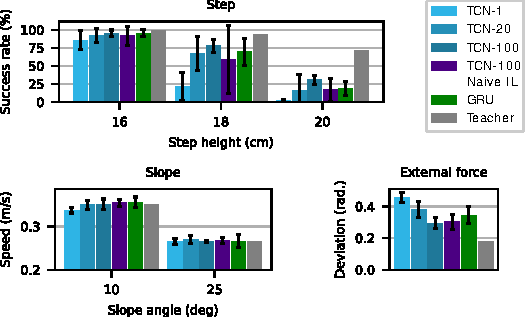
\includegraphics[width=3.5 in]{img/figureS3.pdf}
    \caption{\textbf{本体感知控制器的神经网络架构比较。}本文使用不同随机种子对每个模型训练5次。误差条表示95\%置信区间。`TCN-100 naive IL`表示使用无潜在表示损失的朴素模仿学习（公式19）训练的TCN-100网络。}
    \label{fig:supp_student_comparison}
\end{figure*}

\clearpage
\newpage

\begin{table*}
\centering
 \begin{tabular}{|c|c|c|c|}
\hline
 名称 & 时间 \\ \hline
教师策略训练 & $\approx$ \unit[12]{hrs}  \\
学生策略训练 & $\approx$ \unit[4]{hrs} \\
自适应地形课程 & \unit[2.9]{s}   \\
\hline
\end{tabular}
\caption{\textbf{训练计算时间}。学生策略使用TCN-100架构。训练在配备i7-8700K CPU和Geforce RTX 2080 GPU的台式机上进行。} \label{tab:times}
\end{table*}

\begin{table*}
\centering
 \begin{tabular}{|c|c|c|c|c|}
\hline
地形 & 网格尺寸 & 摩擦系数 & 参数（$c_{T}$） & 范围 \\ \hline
\multirow{3}{*}{\textit{丘陵}} & \multirow{3}{*}{\unit[0.2]{m}}  & \multirow{3}{*}{ $\mathcal{N}(0.7, 0.2)$ }  & 粗糙度（$m$） & $[0.0, 0.05]$ \\
 & & & 频率 & $[0.2, 1.0]$ \\
 & & & 振幅（$m$） & $[0.2, 3.0]$ \\ \hline
 \multirow{3}{*}{\textit{光滑丘陵}} & \multirow{3}{*}{\unit[0.2]{m}}  & \multirow{3}{*}{$\mathcal{N}(0.3, 0.1)$ }  & 粗糙度（$m$） & $[0.0, 0.05]$ \\
 & & & 频率 & $[0.2, 1.0]$ \\
 & & & 振幅（$m$） & $[0.2, 3.0]$ \\ \hline
 \multirow{2}{*}{\textit{台阶}}  & \multirow{2}{*}{\unit[0.02]{m}}  & \multirow{2}{*}{$\mathcal{N}(0.7, 0.2)$}  & 台阶宽度（$m$） & $[0.1, 0.5]$ \\
& & & 台阶高度（$m$） & $[0.05, 0.3]$ \\ \hline
  \multirow{2}{*}{\textit{楼梯}}  & \multirow{2}{*}{\unit[0.02]{m}}  & \multirow{2}{*}{$\mathcal{N}(0.7, 0.2)$}  & 台阶宽度（$m$） & $[0.1, 0.5]$ \\
& & & 台阶高度（$m$） & $[0.02, 0.2]$ \\ \hline
\end{tabular}
\caption{\textbf{仿真地形的参数空间$\mathcal{C}$。} $\mathcal{N}(m, d)$表示该值从均值为$m$、标准差为$d$的高斯分布中采样。摩擦系数裁剪至0.1以上。} \label{tab:terrainparams}
\end{table*}

\begin{table*}
    \centering
    \begin{tabular}{|c|c|} \hline
        参数 & 值 \\ \hline
        粒子数（$N_{particle}$） & 每种地形类型10个 \\ \hline
        转移概率（$p_{transition}$） & 0.8 \\ \hline
        每个粒子的轨迹数（$N_{traj}$） & 6 \\ \hline
        地形参数更新率（$N_{evaluate}$） & 10 \\ \hline
        从回放记忆中采样的概率（$P_{replay}$） & 0.05 \\ \hline
    \end{tabular}
    \caption{\textbf{自动地形课程的超参数。}}
    \label{tab:pfparams}
\end{table*}

\begin{table*}
\centering
 \begin{tabular}{|l|c|c|c|c|}
 \hline
数据 & 维度 & $x_{t}$ &$o_{t}$ &$h_{t}$ \\
\hline
                期望方向（$(^{B}_{IB} \hat{v}_{d})_{xy}$） & 2 &  & \checkmark & \checkmark \\
                期望转向方向（$(^{B}_{IB}\hat{\omega}_{d})_{z}$） & 1 &  & \checkmark & \checkmark \\
                重力向量（$e_g$） & 3 &  & \checkmark & \checkmark \\
                基座角速度（$^{B}_{IB} \omega$） & 3 &  & \checkmark & \checkmark \\
                基座线速度（$^{B}_{IB} v$） & 3 &  & \checkmark & \checkmark \\
                关节位置/速度（$\theta_{i}$, $\dot{\theta_{i}}$） & 24 &  & \checkmark & \checkmark \\
                FTG相位（$\sin(\phi_i)$, $\cos(\phi_i)$） & 8 &  & \checkmark & \checkmark \\
                FTG频率（$\dot{\phi}_i$） & 4 &  & \checkmark & \checkmark \\
                基频（$f_o$） & 1 & &\checkmark &  \\
                关节位置误差历史 & 24 &  &  \checkmark  & \\
                关节速度历史 & 24 &  &  \checkmark  & \\
                足部目标历史（$(r_{f,d})_{t-1, t-2}$） & 24 &  & \checkmark  &  \\
 \hline
                每个足部处的地形法线 & 12 & \checkmark & & \\
                每个足部周围的高度扫描 & 36 & \checkmark & & \\
                足部接触力 & 4 & \checkmark & & \\
                足部接触状态 & 4 & \checkmark & & \\
                大腿接触状态 & 4 & \checkmark & & \\
                小腿接触状态 & 4 & \checkmark & & \\
                足地摩擦系数 & 4 & \checkmark & & \\
                施加在基座上的外部力 & 3 & \checkmark & & \\
 \hline
 \end{tabular}
  \caption{\textbf{本体感知控制器的状态表示（上）和特权信息（下）。}} \label{tab:inputs}
\end{table*}

\begin{table*}
\centering
 \begin{tabular}{|c|c|c|c|c|c|c|c|}
\hline
层 & \multicolumn{2}{|c|}{教师} &  \multicolumn{2}{|c|}{TCN-N学生} & \multicolumn{2}{|c|}{GRU学生}  & {解码器} \\ \hline
输入 & $o_t$ & $x_t$ & $o_t$ & $h$ (60$\times$N) & $o_t$ & $o_t$ & {$\langle o_t, l_t \rangle$} \\ \hline
1 & id & tanh(72) & id & 1D conv dilation 1 & id & GRU(68)  & {relu(196)} \\ \hline
2 & id & tanh(64) & id & 1D conv stride 2 & \multicolumn{2}{|c|}{concatenate} & {Output} \\ \hline
3 & \multicolumn{2}{|c|}{concatenate }& id & 1D conv dilation 2 &  \multicolumn{2}{|c|}{tanh(256)*}  & {-} \\ \hline
4 &  \multicolumn{2}{|c|}{tanh(256)*}  &  id &  1D conv stride 2 &  \multicolumn{2}{|c|}{tanh(128)*} & {-}\\ \hline
5 & \multicolumn{2}{|c|}{tanh(128)*} & id &  1D conv dilation 4  &\multicolumn{2}{|c|}{tanh(64)*} & {-}\\ \hline
6 & \multicolumn{2}{|c|}{tanh(64)*} & id &  1D conv stride 2 & \multicolumn{2}{|c|}{Output*} & {-} \\ \hline
7 &  \multicolumn{2}{|c|}{Output*} & id & tanh(64) & \multicolumn{2}{|c|}{-} & {-} \\ \hline
8 &  \multicolumn{2}{|c|}{-} & \multicolumn{2}{|c|}{concatenate} & \multicolumn{2}{|c|}{-} & {-} \\ \hline
9 &  \multicolumn{2}{|c|}{-} & \multicolumn{2}{|c|}{tanh(256)*} & \multicolumn{2}{|c|}{-} & {-} \\ \hline
10 &  \multicolumn{2}{|c|}{-} & \multicolumn{2}{|c|}{tanh(128)*} & \multicolumn{2}{|c|}{-} & {-} \\ \hline
11 &  \multicolumn{2}{|c|}{-} & \multicolumn{2}{|c|}{tanh(64)*} & \multicolumn{2}{|c|}{-} & {-} \\ \hline
12 &  \multicolumn{2}{|c|}{-} & \multicolumn{2}{|c|}{Output*} & \multicolumn{2}{|c|}{-} & {-} \\ \hline
 \end{tabular}
 \caption{\textbf{神经网络架构。}除非另有说明，卷积层的膨胀率和步长均为1。滤波器大小固定为5。标有$*$的层在教师训练后从教师复制到学习者。id指恒等映射。TCN-N架构使用膨胀因果卷积~\cite{bai2018empirical}。每个卷积层后接relu激活函数。}  \label{tab:netarchitectures}
\end{table*}
\begin{table*}
\centering
 \begin{tabular}{|c|c|c|c|c|c|}
\hline
 模型 & 序列长度 & 通道数 & 参数量 & SGD时间（s） \\ \hline
TCN-1  & 1 & 60 & 161960 & 9.22e-3 ($\pm$1.78e-3)\\ \hline
 TCN-20 & 20 & 44 & 158300 & 2.11e-2 ($\pm$1.24e-3)\\ \hline
 TCN-100 & 100 & 34 & 158070& 5.07e-2 ($\pm$1.94e-3)\\ \hline
 GRU & 100* & - & 159640 & 1.52e-1 ($\pm$1.89e-2) \\ \hline
\end{tabular}
\caption{\textbf{学生策略的网络参数设置及训练时间。} SGD时间指在表S8给出的批次大小下进行一次随机梯度下降更新所需的计算时间。计算时间以经验均值和标准差呈现。*GRU网络的序列长度指用于截断时间反向传播（Truncated BPTT）~\cite{williams1990efficient}的序列长度。} \label{tab:netarchitectures2}
\end{table*}

\begin{table*}
\centering
 \begin{tabular}{|c|c|}
\hline
 参数 & 值  \\ \hline
 折扣因子 & 0.995 \\ \hline
 KL散度阈值 & 0.01  \\ \hline
 最大回合长度 & 400 \\ \hline
 CG阻尼 & 1e-1 \\ \hline
 CG迭代 & 50 \\ \hline
 折扣因子 & 0.995 \\ \hline
批次大小 & 80000 \\ \hline
总迭代次数 & 10000 \\ \hline
\end{tabular}
\caption{\textbf{教师策略训练的超参数。}}
\label{tab:hyperparametersteacher}
\end{table*}

\begin{table*}
\centering
 \begin{tabular}{|c|c|c|}
\hline
 参数 & TCN-N & GRU  \\ \hline
初始学习率 & 5e-4 & 2e-4 \\ \hline
学习率衰减 & \multicolumn{2}{|c|}{exp(0.995, 100)} \\ \hline
 最大回合长度 &\multicolumn{2}{|c|}{400} \\ \hline
 批次大小 & 20000& 10000 \\ \hline
 小批量数 & \multicolumn{2}{|c|}{5} \\ \hline
 训练代数 &\multicolumn{2}{|c|}{4}\\ \hline
 总迭代次数 &\multicolumn{2}{|c|}{4000}\\ \hline
\end{tabular}
\caption{\textbf{学生策略训练的超参数。} exp(a,b)表示指数衰减，定义为$lr_0 * a^{updates/b}$。使用Adam~\cite{kingma2014adam}优化器。}
 \label{tab:hyperparameterslearner}
\end{table*}

\begin{table*}
\centering
 \begin{tabular}{|c|c|}
\hline
 参数 & 值 \\ \hline
初始学习率 & 1e-4 \\ \hline
学习率衰减 & exp(0.99, 100) \\ \hline
 批次大小 & 20000 \\ \hline
 小批量数 & 2\\ \hline
 训练代数 & 10\\ \hline
 总迭代次数 & 1000\\ \hline
 权重衰减 & $l2$-norm, 1e-4 \\ \hline
\end{tabular}
\caption{\textbf{解码器训练的超参数。} exp(a,b)表示指数衰减，定义为$lr_0 * a^{updates/b}$。使用Adam~\cite{kingma2014adam}优化器。}
 \label{tab:hyperparametersdecoder}
\end{table*}


\end{document}